\documentclass[11pt,a4paper]{ctexart}
% Shared preamble for the assignment reports. Use with:
%   \documentclass[11pt,a4paper]{ctexart}  (XeLaTeX)
%   % Shared preamble for the assignment reports. Use with:
%   \documentclass[11pt,a4paper]{ctexart}  (XeLaTeX)
%   % Shared preamble for the assignment reports. Use with:
%   \documentclass[11pt,a4paper]{ctexart}  (XeLaTeX)
%   \input{../common/preamble.tex}
\usepackage[margin=2.3cm]{geometry}
\setmainfont{texgyretermes}[Extension=.otf,UprightFont=*-regular,BoldFont=*-bold,ItalicFont=*-italic,BoldItalicFont=*-bolditalic]
\setsansfont{texgyreheros}[Extension=.otf,UprightFont=*-regular,BoldFont=*-bold,ItalicFont=*-italic,BoldItalicFont=*-bolditalic]
\setmonofont{texgyrecursor}[Extension=.otf,UprightFont=*-regular,BoldFont=*-bold,ItalicFont=*-italic,BoldItalicFont=*-bolditalic]
\usepackage{amsmath,amssymb,mathtools,bm}
\usepackage{graphicx}
\usepackage{booktabs,multirow,makecell,array,tabularx}
\usepackage[table]{xcolor}
\usepackage[most]{tcolorbox}
\usepackage{enumitem}
\usepackage{listings}
\usepackage{subcaption}
\usepackage{siunitx}
\usepackage[hidelinks]{hyperref}
\usepackage[nameinlink,noabbrev]{cleveref}
\usepackage{float}

\setlength{\emergencystretch}{3em}
\linespread{1.15}
\setlist{leftmargin=*,itemsep=2pt,topsep=3pt}
\graphicspath{{figures/}}

\crefname{figure}{图}{图}
\crefname{table}{表}{表}
\crefname{section}{第}{第}
\creflabelformat{section}{#2#1#3 节}
\crefname{equation}{式}{式}
\crefformat{equation}{式~(#2#1#3)}

\lstset{basicstyle=\ttfamily\footnotesize,columns=fullflexible,breaklines=true,frame=single,
  framerule=0.3pt,rulecolor=\color{black!40},backgroundcolor=\color{black!3},
  keywordstyle=\color{blue!60!black}\bfseries,commentstyle=\color{green!40!black},
  numbers=left,numberstyle=\tiny\color{black!50},xleftmargin=1.5em}

% Interview boxes: question, model answer, common wrong answer.
\newtcolorbox{iqbox}[1]{enhanced,breakable,colback=blue!3,colframe=blue!45!black,boxrule=0.5pt,arc=1.5pt,
  left=4pt,right=4pt,top=3pt,bottom=3pt,fonttitle=\bfseries\small,title={面试追问：#1}}
\newtcolorbox{findingbox}[1][]{enhanced,breakable,colback=green!3,colframe=green!40!black,boxrule=0.5pt,arc=1.5pt,
  left=4pt,right=4pt,top=3pt,bottom=3pt,fonttitle=\bfseries\small,title={结论#1}}
\newtcolorbox{caveatbox}{enhanced,breakable,colback=orange!4,colframe=orange!60!black,boxrule=0.5pt,arc=1.5pt,
  left=4pt,right=4pt,top=3pt,bottom=3pt,fonttitle=\bfseries\small,title={不能推出的结论}}

\newcommand{\authorline}{ShaneLiu04\thanks{GitHub: \url{https://github.com/ShaneLiu04}。代码与原始指标：\url{https://gitee.com/liu-xingyan04/mlsys-infra}。本文基于公开课程材料独立完成，与课程团队无隶属关系。}}

\usepackage[margin=2.3cm]{geometry}
\setmainfont{texgyretermes}[Extension=.otf,UprightFont=*-regular,BoldFont=*-bold,ItalicFont=*-italic,BoldItalicFont=*-bolditalic]
\setsansfont{texgyreheros}[Extension=.otf,UprightFont=*-regular,BoldFont=*-bold,ItalicFont=*-italic,BoldItalicFont=*-bolditalic]
\setmonofont{texgyrecursor}[Extension=.otf,UprightFont=*-regular,BoldFont=*-bold,ItalicFont=*-italic,BoldItalicFont=*-bolditalic]
\usepackage{amsmath,amssymb,mathtools,bm}
\usepackage{graphicx}
\usepackage{booktabs,multirow,makecell,array,tabularx}
\usepackage[table]{xcolor}
\usepackage[most]{tcolorbox}
\usepackage{enumitem}
\usepackage{listings}
\usepackage{subcaption}
\usepackage{siunitx}
\usepackage[hidelinks]{hyperref}
\usepackage[nameinlink,noabbrev]{cleveref}
\usepackage{float}

\setlength{\emergencystretch}{3em}
\linespread{1.15}
\setlist{leftmargin=*,itemsep=2pt,topsep=3pt}
\graphicspath{{figures/}}

\crefname{figure}{图}{图}
\crefname{table}{表}{表}
\crefname{section}{第}{第}
\creflabelformat{section}{#2#1#3 节}
\crefname{equation}{式}{式}
\crefformat{equation}{式~(#2#1#3)}

\lstset{basicstyle=\ttfamily\footnotesize,columns=fullflexible,breaklines=true,frame=single,
  framerule=0.3pt,rulecolor=\color{black!40},backgroundcolor=\color{black!3},
  keywordstyle=\color{blue!60!black}\bfseries,commentstyle=\color{green!40!black},
  numbers=left,numberstyle=\tiny\color{black!50},xleftmargin=1.5em}

% Interview boxes: question, model answer, common wrong answer.
\newtcolorbox{iqbox}[1]{enhanced,breakable,colback=blue!3,colframe=blue!45!black,boxrule=0.5pt,arc=1.5pt,
  left=4pt,right=4pt,top=3pt,bottom=3pt,fonttitle=\bfseries\small,title={面试追问：#1}}
\newtcolorbox{findingbox}[1][]{enhanced,breakable,colback=green!3,colframe=green!40!black,boxrule=0.5pt,arc=1.5pt,
  left=4pt,right=4pt,top=3pt,bottom=3pt,fonttitle=\bfseries\small,title={结论#1}}
\newtcolorbox{caveatbox}{enhanced,breakable,colback=orange!4,colframe=orange!60!black,boxrule=0.5pt,arc=1.5pt,
  left=4pt,right=4pt,top=3pt,bottom=3pt,fonttitle=\bfseries\small,title={不能推出的结论}}

\newcommand{\authorline}{ShaneLiu04\thanks{GitHub: \url{https://github.com/ShaneLiu04}。代码与原始指标：\url{https://gitee.com/liu-xingyan04/mlsys-infra}。本文基于公开课程材料独立完成，与课程团队无隶属关系。}}

\usepackage[margin=2.3cm]{geometry}
\setmainfont{texgyretermes}[Extension=.otf,UprightFont=*-regular,BoldFont=*-bold,ItalicFont=*-italic,BoldItalicFont=*-bolditalic]
\setsansfont{texgyreheros}[Extension=.otf,UprightFont=*-regular,BoldFont=*-bold,ItalicFont=*-italic,BoldItalicFont=*-bolditalic]
\setmonofont{texgyrecursor}[Extension=.otf,UprightFont=*-regular,BoldFont=*-bold,ItalicFont=*-italic,BoldItalicFont=*-bolditalic]
\usepackage{amsmath,amssymb,mathtools,bm}
\usepackage{graphicx}
\usepackage{booktabs,multirow,makecell,array,tabularx}
\usepackage[table]{xcolor}
\usepackage[most]{tcolorbox}
\usepackage{enumitem}
\usepackage{listings}
\usepackage{subcaption}
\usepackage{siunitx}
\usepackage[hidelinks]{hyperref}
\usepackage[nameinlink,noabbrev]{cleveref}
\usepackage{float}

\setlength{\emergencystretch}{3em}
\linespread{1.15}
\setlist{leftmargin=*,itemsep=2pt,topsep=3pt}
\graphicspath{{figures/}}

\crefname{figure}{图}{图}
\crefname{table}{表}{表}
\crefname{section}{第}{第}
\creflabelformat{section}{#2#1#3 节}
\crefname{equation}{式}{式}
\crefformat{equation}{式~(#2#1#3)}

\lstset{basicstyle=\ttfamily\footnotesize,columns=fullflexible,breaklines=true,frame=single,
  framerule=0.3pt,rulecolor=\color{black!40},backgroundcolor=\color{black!3},
  keywordstyle=\color{blue!60!black}\bfseries,commentstyle=\color{green!40!black},
  numbers=left,numberstyle=\tiny\color{black!50},xleftmargin=1.5em}

% Interview boxes: question, model answer, common wrong answer.
\newtcolorbox{iqbox}[1]{enhanced,breakable,colback=blue!3,colframe=blue!45!black,boxrule=0.5pt,arc=1.5pt,
  left=4pt,right=4pt,top=3pt,bottom=3pt,fonttitle=\bfseries\small,title={面试追问：#1}}
\newtcolorbox{findingbox}[1][]{enhanced,breakable,colback=green!3,colframe=green!40!black,boxrule=0.5pt,arc=1.5pt,
  left=4pt,right=4pt,top=3pt,bottom=3pt,fonttitle=\bfseries\small,title={结论#1}}
\newtcolorbox{caveatbox}{enhanced,breakable,colback=orange!4,colframe=orange!60!black,boxrule=0.5pt,arc=1.5pt,
  left=4pt,right=4pt,top=3pt,bottom=3pt,fonttitle=\bfseries\small,title={不能推出的结论}}

\newcommand{\authorline}{ShaneLiu04\thanks{GitHub: \url{https://github.com/ShaneLiu04}。代码与原始指标：\url{https://gitee.com/liu-xingyan04/mlsys-infra}。本文基于公开课程材料独立完成，与课程团队无隶属关系。}}

\graphicspath{{../../solutions/cs149/asst4-dnn-accelerator/artifacts/figures/}}

\title{CS149 Assignment 4 复现报告：\\DNN 加速器上的分块、数据复用与融合——从 Trainium 模型到 RTX 5090 实测}
\author{\authorline}
\date{2026 年 10 月}

\begin{document}
\maketitle

\begin{abstract}
CS149 Fall 2024 Assignment 4 要求在 AWS Trainium 上用 NKI 写分块矩阵乘，以及融合的 conv2d+maxpool。它真正想让人想清楚的是四件事：
片上存储（SBUF/PSUM）放得下多大的 tile；tile 大小怎样决定算术强度；怎样让 tensor engine 一直有活干；融合能省下多少 HBM 流量。
我们没有 Trainium，所以分两层来回答。第一层是 CPU 上可以测量的模型：带 SBUF/PSUM 容量约束的分块流量与周期模型、寄存器级脉动阵列仿真和 im2col 卷积。
第二层把同一组问题搬到 RTX 5090 上实测，包括 11 级 SGEMM 优化阶梯、WMMA tensor-core GEMM、实测 roofline、skinny（decode 形）GEMM、
直接卷积 / im2col / implicit GEMM / cuDNN 的对比，以及 conv+ReLU+maxpool 融合。

先看硬件上限：RTX 5090 实测 DRAM triad 带宽 1549~GB/s（规格的 86\%），L2 常驻时 5107~GB/s，fp32 FMA 峰值 118.97~TFLOP/s，cuBLAS bf16 232.0~TFLOP/s。
SGEMM 从 naive 的 0.94~TFLOP/s 提升到 float4 寄存器分块的 49.40~TFLOP/s，提高了 52.6 倍，是 fp32 峰值的 41.5\%、cuBLAS fp32 的 78.3\%；
我写的 WMMA fp16 kernel 达到 177.80~TFLOP/s（cuBLAS fp16 的 85.7\%）。最有说服力的一条交叉验证是：CPU 部分的流量公式在 GPU 上直接成立。
8192$^3$ 时 smem8 kernel 的工作集远超 L2，用这个公式反推出的 DRAM 带宽为 1585~GB/s，与实测 triad 只差 2.3\%。
融合的收益取决于中间张量落在哪一级存储：batch 64 时 3$\times$3@112 层的中间张量有 196~MiB，溢出 L2，直接卷积路径融合后模型 DRAM 流量从 1029.1 降到 245.1~MiB，
时间从 4.230 降到 3.768~ms；batch 8 时中间结果留在 L2 里，融合只省 17~µs。ncu 在容器内没有性能计数器权限，
因此 occupancy 和 bank conflict 由 CUDA occupancy API 与解析模型给出，文中会明确标注。
\end{abstract}

\tableofcontents
\newpage

%==========================================================================================
\section{背景与作业要求}

\subsection{官方作业在问什么}
CS149（Stanford Parallel Computing）Fall 2024 的 Assignment 4 题为 \emph{Optimizing DNN Performance on DNN Accelerator Hardware}，
在 AWS Trainium（Trn1 NeuronCore）上用 NKI（Neuron Kernel Interface）编程。官方 handout 的主线大致有三部分：
\begin{enumerate}
  \item NKI 入门与分块 matmul。先理解有 128 个 partition 的 SBUF（片上 scratchpad，由程序显式管理的高速存储）、PSUM（矩阵乘结果的累加缓冲），以及 HBM 与 SBUF 之间的 DMA；
        再把大矩阵乘拆成放得进 SBUF/PSUM 的 tile，调 tile 大小来提高数据复用，让 tensor engine（一个脉动阵列~\cite{kung1982,jouppi2017}）保持忙碌。
  \item 用矩阵乘实现 conv2d：把卷积改写为 GEMM（im2col~\cite{chellapilla2006}，或者按 filter tap 累加），并处理 channel 维度的分块。
  \item 融合 conv2d + maxpool：在片上完成卷积、（可选的偏置和激活）和池化，只把池化后的结果写回 HBM，并分析性能。
\end{enumerate}
具体分值与接口以官方 handout 为准。这份作业里能带到别的硬件上的，是一条推理链和一笔账。推理链是：片上容量决定最大 tile，最大 tile 决定算术强度，
算术强度又决定 kernel 是计算受限还是带宽受限。那笔账是：融合省掉了中间张量写出去再读回来的流量。

\subsection{本仓库的对应方式}
因为手上没有 Trainium，每个官方部分都分成「CPU 上的模型」和「GPU 上的对照」两份来做，对应关系见下表。
\begin{table}[H]
\centering\small
\begin{tabularx}{\linewidth}{>{\raggedright}p{3.4cm}X>{\raggedright\arraybackslash}p{3.6cm}}
\toprule
官方部分 & 本仓库实现 & 对照 \\
\midrule
NKI tile / SBUF / PSUM / DMA & \texttt{code/dnnaccel/tiling.py}：输出驻留 PSUM 的三重循环，精确计 HBM 字节、DMA 次数、周期；容量约束下搜索 tile & GPU：\texttt{gpu/sgemm.cu} 的 shared-memory/寄存器分块~\cite{goto2008}，同一流量公式 \\
tensor engine（脉动阵列） & \texttt{code/dnnaccel/systolic.py}：P$\times$P weight-stationary 寄存器级仿真 & GPU：WMMA tensor core（\texttt{k\_wmma}） \\
分块 matmul 调优 & \texttt{code/dnnaccel/gemm\_cpu.py}（CPU 计时） & 11 级 SGEMM 阶梯、tile 热力图、cuBLAS 多精度对照 \\
conv2d 改写为 GEMM & \texttt{code/dnnaccel/im2col.py}（numpy） & \texttt{gpu/conv.cu}：直接卷积、显式 im2col+cuBLAS、implicit GEMM、cuDNN~\cite{chetlur2014} \\
融合 conv + maxpool & （CPU 部分未做） & \texttt{k\_conv2x2<FUSE>}：ReLU+maxpool 在寄存器里完成；对照 3 个 kernel 的非融合版 \\
性能分析 & 模型 roofline~\cite{williams2009}（假设参数） & 实测 roofline（copy/triad~\cite{mccalpin1995}、FMA 链、cuBLAS bf16） \\
\bottomrule
\end{tabularx}
\caption{官方作业各部分与本仓库实现的对应。}
\end{table}

GPU 和 Trainium 的概念可以大致对上：shared memory（每 SM 最多约 100~KB 可分配给一个 block）相当于 SBUF；
寄存器文件里的累加器（每 SM 64K 个 32 位寄存器，即 256~KB）相当于 PSUM；tensor core 相当于 PE 阵列；
\texttt{cp.async} 双缓冲相当于让 DMA 与计算重叠。有一样东西在 Trainium 模型里没有对应：96~MB 的 L2。后文会反复看到，
很多「按 DRAM 算应该是带宽受限」的 kernel 实际跑得比模型快，原因就在这块 L2。

%==========================================================================================
\section{实验环境}

CPU 部分在本地机器上跑，GPU 部分在 AutoDL 的容器里跑，两边的配置见下表。

\begin{table}[H]
\centering\small
\begin{tabularx}{\linewidth}{lXX}
\toprule
 & CPU 部分（本地） & GPU 部分（AutoDL 容器） \\
\midrule
处理器 & Intel64 Family 6 Model 106，4 物理核 / 8 逻辑核，与其他任务共享 & NVIDIA GeForce RTX 5090，170 SM，sm\_120 \\
存储 & — & 32 GB GDDR7（规格 1792 GB/s），L2 96 MB \\
时钟/功耗 & — & 最大 SM 时钟 3090 MHz，显存 14001 MHz，功耗上限 575 W \\
软件 & Python 3.12.10，numpy 2.5.3，torch 2.6 CPU & Python 3.12.3，torch 2.8.0+cu128，CUDA 12.8，cuDNN 91002 \\
编译 & — & \texttt{nvcc -O3 -arch=sm\_120 -shared -Xcompiler -fPIC}，驱动 595.71.05 \\
CPU 绑定 & — & \texttt{taskset -c 36,37}，\texttt{OMP\_NUM\_THREADS=2} \\
\bottomrule
\end{tabularx}
\caption{实验环境。GPU 元数据见 \texttt{artifacts/raw/gpu/meta\_gpu.json}，CPU 见 \texttt{artifacts/raw/meta.json}。}
\end{table}

加速器模型用的参数（128$\times$128 PE、1.4~GHz、HBM 410~GB/s、SBUF 24~MiB、PSUM 2~MiB、每次 DMA 固定 1~µs）是\textbf{假设}，
不是 Trainium 的规格表。按这组参数，峰值为 45.88~TFLOP/s，ridge（算力受限与带宽受限的分界强度）为 111.9~FLOP/B。
GPU 所在的机器同时还有另外 6 个任务，所以所有 GPU 计时都在一把文件锁（\texttt{flock}）下独占进行。

%==========================================================================================
\section{方法与实现}

这一节先讲 CPU 侧的模型怎么算流量，再讲 GPU 侧每个 kernel 改了什么、怎么计时。两侧用的是同一个流量公式，这是后面能做交叉验证的前提。

\subsection{CPU 侧：分块流量与周期模型}
\texttt{tiling.py} 模拟的是输出驻留（output-stationary~\cite{chen2017eyeriss}，即输出 tile 一直留在累加缓冲里，直到算完才写回）的循环：
\begin{lstlisting}[language=Python]
for i in M/tm:            # C row block
  for j in N/tn:          # C col block
    for k in K/tk:        # DMA A[i,k] (tm x tk), B[k,j] (tk x tn) into SBUF
      PSUM[i,j] += A[i,k] @ B[k,j]
    DMA PSUM[i,j] -> HBM
\end{lstlisting}
在这个循环里，每个 A 元素被每个列块读一次，每个 B 元素被每个行块读一次，于是
\begin{equation}
\begin{aligned}
\text{HBM bytes} &= b\left(MK\left\lceil N/t_n\right\rceil + KN\left\lceil M/t_m\right\rceil + MN\right),\\
I &= \frac{2MNK}{\text{HBM bytes}} \xrightarrow{M,N,K\gg t} \frac{2}{b(1/t_m+1/t_n)} .
\end{aligned}
\label{eq:traffic}
\end{equation}
容量约束有两条：SBUF 要放下双缓冲的 A、B 块，即 $2b\,t_k(t_m+t_n)\le \text{SBUF}$；PSUM 要放下 fp32 累加的输出块~\cite{micikevicius2018}，即 $4\,t_m t_n\le\text{PSUM}$。
测试里用 numpy 实际执行同一个循环，逐字节核对计数与公式相等。脉动阵列仿真则按寄存器逐周期推进，每个权重块需要 $M+2P-2$ 个周期。

\subsection{GPU 侧：SGEMM 阶梯}
所有 kernel 都写在 \texttt{gpu/sgemm.cu} 里，编译成共享库，用 \texttt{ctypes} 从 Python 调用，直接传 torch 张量的设备指针。
这样做的好处是，参考结果、计时（\texttt{torch.cuda.Event}）和 cuBLAS 对照都在同一个进程、同一条默认流上。阶梯的每一级只改一件事（行主序 $C=AB$）：
\begin{description}[leftmargin=1.5em]
  \item[naive] \texttt{threadIdx.x} 对应行。一个 warp 读 32 个不同行的 A（跨度 $K$），写 C 也跨行，访存完全不合并。
  \item[coalesced] \texttt{threadIdx.x} 改为对应列。B 的读和 C 的写在 warp 内变成连续地址，A 变成广播。
  \item[smem8/16/32] 经典的 $T\times T$ shared-memory 分块，每个线程算 1 个输出。
  \item[reg1d] 块 64$\times$64、BK=8，每个线程算同一列的 8 行（TM=8），512 线程。
  \item[reg2d] 块 128$\times$128、BK=8，每个线程算 8$\times$8，256 线程；A 在 smem 里转置存放。加载循环是通用的标量写法，可以实例化任意 BM、BN，热力图就用它。
  \item[reg2d\_nc] 同上，但 As 每行补 4 个 float，线程负责的 8 列按 16 跨步分布，用来消除 bank conflict。
  \item[vec4] reg2d 的 128$\times$128 版本，改用 float4 全局读、LDS.128~\cite{jia2018}（一条指令读 128 位）的 shared 读和 float4 写回。
  \item[vec4\_db] 再加两级 smem 缓冲：下一个 tile 先读进寄存器，算完当前 tile 再写进另一级 smem，这样每个 k 步只需一次 \texttt{\_\_syncthreads}。
  \item[vec4\_db\_lb2] 同上，加 \texttt{\_\_launch\_bounds\_\_(256,2)}。
  \item[skinny] 面向 $M\le 64$ 的 decode 形 GEMM。每个线程负责一列，A 的 8 行放进 smem 广播，K 维拆给多个 block（split-K），结果用 \texttt{atomicAdd} 累加。
  \item[wmma] fp16/bf16 输入、fp32 累加。块 128$\times$128$\times$32，8 个 warp 排成 2$\times$4，每个 warp 负责 64$\times$32（4$\times$2 个 16$\times$16 fragment）；
        两级 smem 由 \texttt{cp.async} 填充，与 MMA 重叠。
\end{description}

\cref{lst:vec} 是 vec4 的内层循环。每个 k 步，每个线程用 4 条 LDS.128 喂 64 条 FMA，后文会看到这个比例有多重要。
\begin{lstlisting}[language=C++,caption={vec4 内层循环（\texttt{gpu/sgemm.cu}）},label=lst:vec]
for (int k = 0; k < BK; ++k) {
  float4 a0 = *reinterpret_cast<const float4*>(&As[st][k][trow * TM]);
  float4 a1 = *reinterpret_cast<const float4*>(&As[st][k][trow * TM + 4]);
  float4 b0 = *reinterpret_cast<const float4*>(&Bs[st][k][tcol * TN]);
  float4 b1 = *reinterpret_cast<const float4*>(&Bs[st][k][tcol * TN + 4]);
  /* unpack into ra[8], rb[8] */
  for (int i = 0; i < TM; ++i)
    for (int j = 0; j < TN; ++j) acc[i][j] += ra[i] * rb[j];   // 64 FMA
}
\end{lstlisting}

\cref{lst:wmma} 是 WMMA kernel 的主循环：先等上一级 \texttt{cp.async} 完成，立刻发起下一级的异步拷贝，再在当前这一级上做 MMA。
它和 NKI 里「DMA 搬下一个 tile 的同时，tensor engine 算当前 tile」是同一个结构。
\begin{lstlisting}[language=C++,caption={WMMA 主循环（\texttt{gpu/sgemm.cu}）},label=lst:wmma]
load(0, 0);
for (int k0 = 0; k0 < K; k0 += BK) {
  cp_async_wait0();
  __syncthreads();
  if (k0 + BK < K) load(st ^ 1, k0 + BK);      // prefetch next stage
  for (int kk = 0; kk < BK; kk += 16) {
    wm::load_matrix_sync(fa[i], &As[st][wm_ * 64 + i * 16][kk], BK + PADA);   // i = 0..3
    wm::load_matrix_sync(fb[j], &Bs[st][kk][wn_ * 32 + j * 16], BN + PADB);   // j = 0..1
    wm::mma_sync(acc[i][j], fa[i], fb[j], acc[i][j]);                         // 8 MMAs
  }
  __syncthreads();
  st ^= 1;
}
\end{lstlisting}

\subsection{Roofline 微基准}
要判断一个 kernel 离上限多远，得先知道上限在哪里。\texttt{gpu/micro.cu} 用三类微基准量出几个屋顶。
带宽屋顶用 grid-stride 的 float4 copy（$2n\cdot4$ 字节）和 triad $a=b+s\,c$（$3n\cdot4$ 字节），数组大小从 4~MiB 到 1~GiB，这样能同时测到 L2 和 DRAM 两层。
fp32 算力屋顶用 FMA 链 kernel：每个线程跑 $C\in\{1,2,4,8,16\}$ 条相互独立的 \texttt{fmaf} 链、各 4096 次迭代，扫描线程数和每 SM 的 block 数，取最大值。
tensor-core 屋顶则取 cuBLAS bf16/fp16/tf32 在 4096--16384 方阵上的最大值。

\subsection{卷积与融合}
\texttt{gpu/conv.cu} 实现了几种卷积（NCHW 布局，fp32）：
\begin{itemize}
  \item direct：每个线程算一个输出，循环 $C\cdot K_H\cdot K_W$ 次。
  \item 显式 im2col：一个 kernel 生成 \texttt{cols[n][c·KH·KW][oh·OW+ow]}，再用 \texttt{torch.matmul}（cuBLAS fp32）乘以 $W\in\mathbb{R}^{F\times CK_HK_W}$；同时记录缓冲区字节数和峰值显存增量。
  \item implicit GEMM：从 GEMM 的角度看，$M=F$、$N=N_b\cdot OH\cdot OW$、$K=CK_HK_W$。B tile 在装进 smem 时现场从 $x$ 里 gather，不物化 im2col 矩阵。块 64$\times$128，每个线程算 8$\times$8。
  \item 融合 conv+ReLU+maxpool，见\cref{lst:fuse}。每个线程算一个池化窗口对应的 2$\times$2 个卷积输出，并同时处理 8 个 filter，让输入像素在寄存器里复用 8 次。
        \texttt{FUSE=true} 时，在寄存器里取 max 和 ReLU，只写出 1 个值；\texttt{FUSE=false} 时写出 4 个原始输出，再交给独立的 ReLU kernel 和 maxpool kernel。
        两条路径的卷积计算完全相同，唯一的差别是中间张量有没有落到显存，这样比出来的就只是融合本身的收益。
\end{itemize}
\begin{lstlisting}[language=C++,caption={融合 epilogue（\texttt{k\_conv2x2<FUSE, FT>}）},label=lst:fuse]
for (int t = 0; t < FT; ++t) {
  if (FUSE) {
    float m = fmaxf(fmaxf(acc[t][0], acc[t][1]), fmaxf(acc[t][2], acc[t][3]));
    y[(((size_t)n * s.F + f) * PH + py) * PW + px] = fmaxf(m, 0.f);   // 1 store
  } else {
    float* yo = y + (((size_t)n * s.F + f) * s.OH + oh0) * s.OW + ow0;
    yo[0] = acc[t][0]; yo[1] = acc[t][1]; yo[s.OW] = acc[t][2]; yo[s.OW + 1] = acc[t][3];
  }
}
\end{lstlisting}
另外还有两组对照：cuDNN conv + \texttt{F.relu} + \texttt{F.max\_pool2d}（3 个 kernel）对比 cuDNN conv + 我的融合 ReLU-pool kernel；
以及我的 implicit GEMM（ReLU 融合进 epilogue）+ pool。融合实验在 batch 8 和 batch 64 各跑一次。

\subsection{测量方法}
GPU 上的数字很容易被测量方式带偏，下面几条口径决定了后面的数字能不能信：
\begin{itemize}
  \item 计时：先热身一次，再按估计耗时决定重复次数（目标总时长 0.08~s，3--100 次）。每次用一对 cudaEvent，取中位数。
  \item cold L2：skinny GEMM 额外跑一遍「冷 L2」，每次计时前写一个 256~MiB 的缓冲区把 L2 冲掉（写入在事件窗口之外）。
  \item 误差：取 $\max|C-C_{\mathrm{fp64}}|/\max|C_{\mathrm{fp64}}|$。参考结果用 fp64 在\emph{同一组已舍入的输入}上计算（fp16/bf16/fp8~\cite{micikevicius2022} 先舍入再升精度），
        所以误差只反映累加和输出的舍入，不含输入量化。
  \item TF32：fp32 基线显式关闭 \texttt{allow\_tf32}，因为 cuDNN 默认是开的。第一轮融合实验我漏关了，结果 cuDNN 的误差冒出 $3\times10^{-4}$，这才发现问题，之后全部重跑。
  \item ncu 的替代：\texttt{ncu} 返回 \texttt{ERR\_NVGPUCTRPERM}（容器没有性能计数器权限，见 \texttt{ncu\_raw.csv}），按要求只尝试一次。
        替代方案是用 \texttt{cudaFuncGetAttributes} 与 \texttt{cudaOccupancy\-MaxActive\-Blocks\-PerMultiprocessor} 给出寄存器、静态 smem 和理论 occupancy（\texttt{kernel\_info.jsonl}），
        用 \texttt{-Xptxas -v} 给出 spill（\texttt{ptxas\_sgemm.txt}），用解析模型 \texttt{gpu/bankmodel.py} 估计 bank conflict 的程度（\texttt{bank\_model.jsonl}）。
\end{itemize}

\subsection{正确性}
\texttt{tests/test\_gpu.py} 在 GPU 上覆盖了这些组合：11 个 SGEMM 变体 $\times$ 3 种形状（含非 128 倍数的 200$\times$136$\times$72）、3 种 reg2d tile、skinny 的 4 个 $M$、
WMMA fp16/bf16、4 种卷积形状（7$\times$7/2、3$\times$3、1$\times$1、3$\times$3/2）的 direct/implicit/im2col，以及融合与非融合的 conv+ReLU+pool。
服务器上 66 个测试全部通过，3 个跳过（vec4 系列不支持非 128 倍数的形状）。本地没有 CUDA 时 GPU 模块整体跳过，CPU 侧 21 个测试通过。

%==========================================================================================
\section{实验结果}

结果按「先模型、后实测」的顺序展开：先在 CPU 模型里看清 tile、容量和强度的关系，再到 GPU 上检验这些关系还成不成立。

\subsection{CPU 模型：tile 大小、容量与算术强度}
第一个问题是：tile 变大，强度涨多少？涨到哪里会停？
\begin{figure}[H]
\centering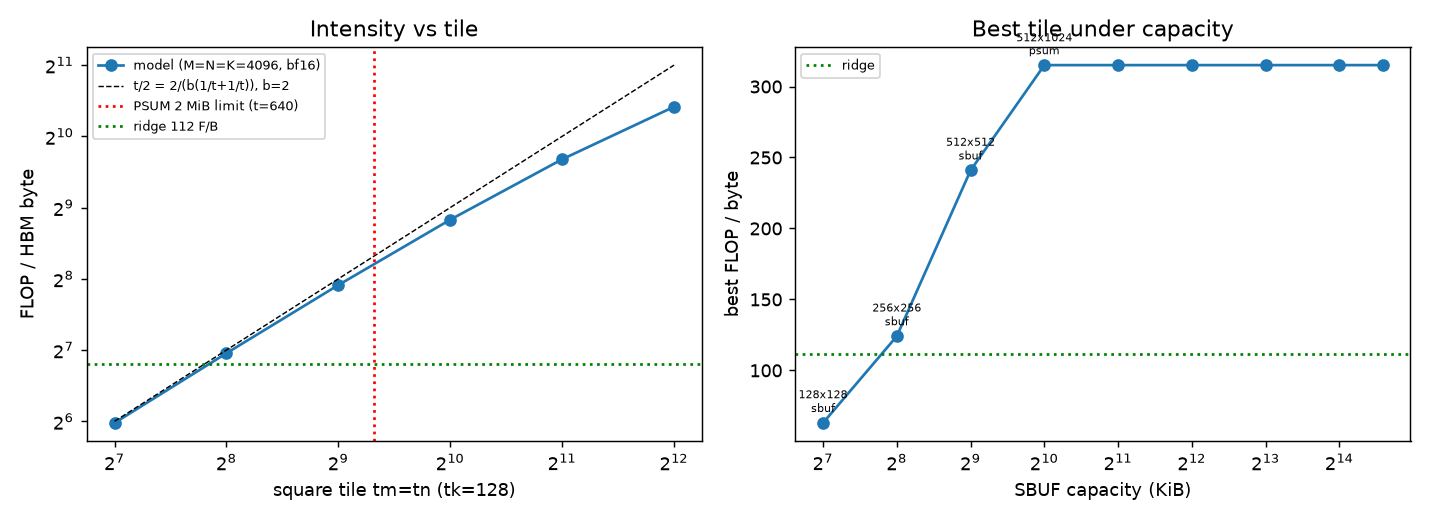
\includegraphics[width=\linewidth]{tiling_intensity.png}
\caption{左：M=N=K=4096、bf16 时 HBM 算术强度随方形 tile 边长变化，虚线为 $t/2$；右：给定 SBUF 容量时搜索到的最优 tile 的强度（PSUM 固定 2~MiB）。数据：\texttt{tiling\_square.csv}、\texttt{tiling\_capacity.csv}。}
\label{fig:tiling}
\end{figure}
\Cref{fig:tiling} 左图的点几乎都落在 $t/2$ 虚线上：tile 为 128、256、512 时，强度分别是 63.02、124.12、240.94~FLOP/B，正是 \cref{eq:traffic} 在 $b=2$ 时给出的 $t/b$。
右图说明强度在哪里停下。SBUF $\le$ 512~KiB 时，先满的是 SBUF（\texttt{sbuf\_used}=1.0）；到 $\ge$1~MiB 之后，先满的变成 2~MiB 的 PSUM，tile 停在 512$\times$1024，强度停在 315.08~FLOP/B。
再往后加 SBUF，只会让 $t_k$ 变大，DMA 次数从 2080 降到 96，强度却不变。
原因在公式里：强度由输出 tile 的面积决定，而输出 tile 受累加缓冲的容量限制；$t_k$ 只影响 DMA 次数和固定开销。
GPU 上也是这样，累加器住在寄存器文件里，寄存器文件决定了 block tile 的上限（见 \cref{sec:theory}）。

\begin{findingbox}[：PSUM 而不是 SBUF 决定强度上限]
模型中 SBUF 从 1~MiB 增加到 24~MiB，最优强度一直是 315.08~FLOP/B；只有 PSUM 变大，tile 才能做大。
\end{findingbox}

\subsection{CPU 模型：脉动阵列利用率}
tile 够大之后，还要让 tensor engine 一直忙。脉动阵列每处理一个权重块都要先填满、再排空，这段开销能不能摊薄，取决于矩阵够不够大。
\begin{figure}[H]
\centering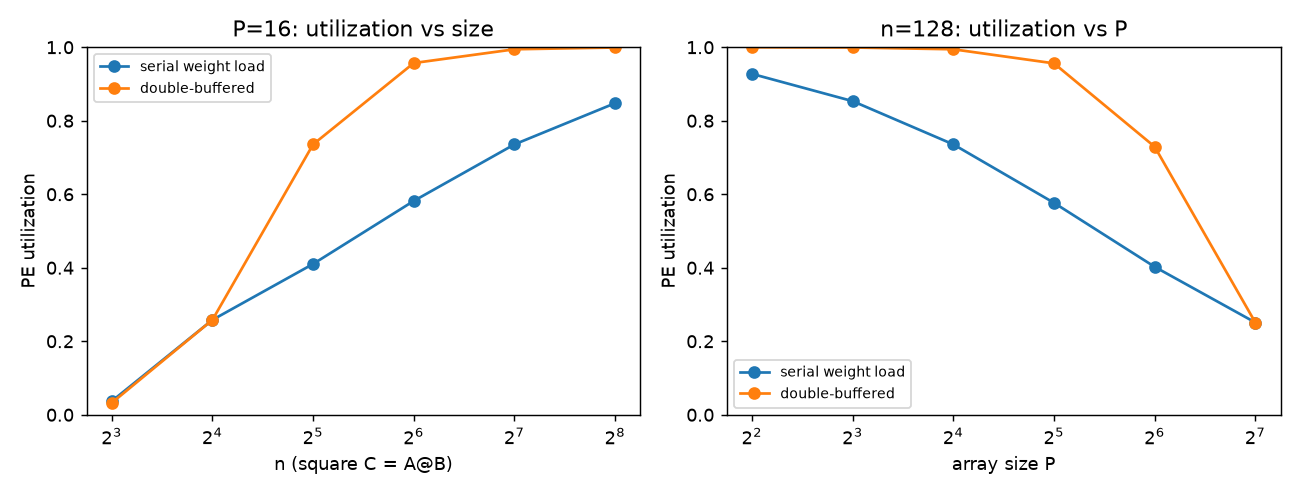
\includegraphics[width=0.92\linewidth]{systolic_utilization.png}
\caption{weight-stationary 脉动阵列的 PE 利用率。左：P=16 时随矩阵规模；右：n=128 时随阵列边长 P。数据：\texttt{systolic\_vs\_size.csv}、\texttt{systolic\_vs\_p.csv}。}
\label{fig:systolic}
\end{figure}
每个权重块需要 $M+2P-2$ 个周期：$M$ 行数据流入，再加 $2(P-1)$ 个周期的填充与排空。P=16、n=256 时，串行加载权重的利用率是 0.848，权重双缓冲后升到 0.999。
但 n=128 时，P 从 4 增加到 128，串行利用率从 0.928 跌到 0.251，双缓冲也救不回来，仍是 0.251，因为矩阵只有一个块，没有下一个块可以衔接。
所以阵列越大，越需要大矩阵来摊薄 $3P-2$ 的开销。GPU 上「小矩阵只能用到少数 SM」（\cref{sec:ladder} 的 256$^3$ 结果）是同一类现象：并行单元越大，越需要足够多的独立工作。

\subsection{CPU 实测 GEMM}
模型之外，CPU 上也实测了几种 GEMM 写法，看看分块在真实机器上能带来什么。
\begin{figure}[H]
\centering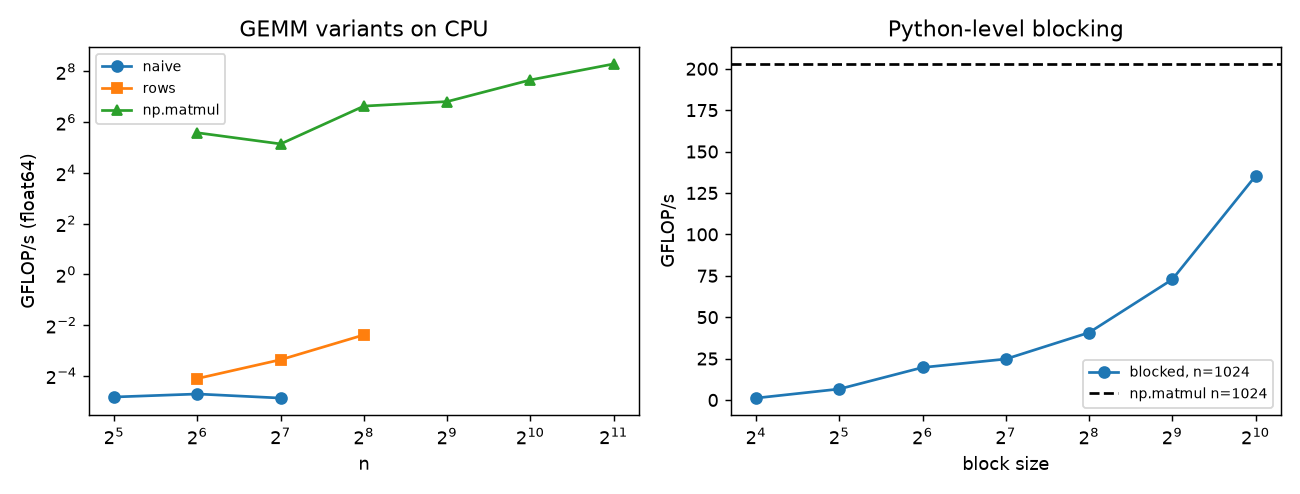
\includegraphics[width=0.92\linewidth]{cpu_gemm.png}
\caption{CPU float64 GEMM。左：纯 Python、行向量 AXPY、\texttt{np.matmul}；右：Python 级分块随块大小（n=1024）。数据：\texttt{cpu\_gemm.csv}。}
\label{fig:cpugemm}
\end{figure}
\texttt{np.matmul} 在 n=2048 时达到 314.3~GFLOP/s，纯 Python 三重循环在 n=128 时只有 0.034~GFLOP/s，相差约 9200 倍。
Python 级分块在 bs=16、64、1024 时分别为 1.16、19.6、135.3~GFLOP/s。块越小越慢，是因为要做 $(n/bs)^3$ 次调用，解释器开销随之暴涨，而不是 cache 失效。
也就是说，在 CPU 上分块的收益被调用开销盖住了；到了 GPU 上，没有这层开销，分块直接决定 DRAM 流量和性能。

\subsection{CPU 实测 im2col}
im2col 把卷积变成 GEMM，代价是要把输入 patch 展开成一个大矩阵。这个矩阵有多大？
\begin{figure}[H]
\centering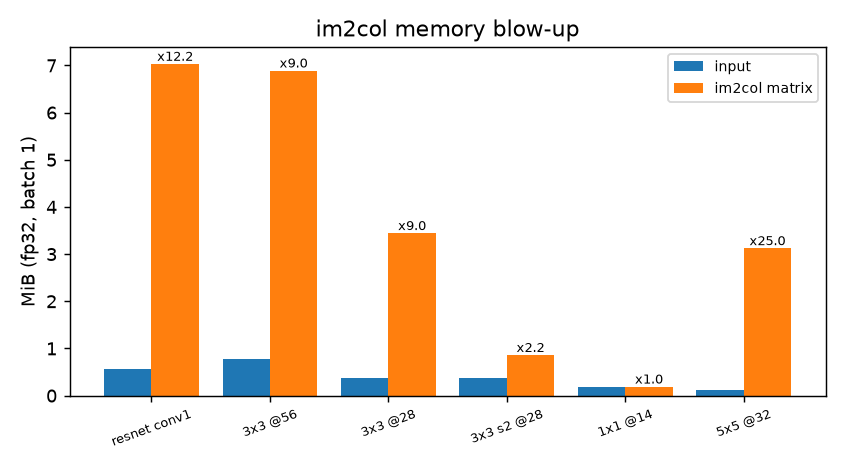
\includegraphics[width=0.7\linewidth]{im2col_blowup.png}
\caption{im2col 的内存膨胀（fp32，batch 1，CPU）。数据：\texttt{im2col.csv}。}
\label{fig:im2colcpu}
\end{figure}
膨胀倍数约为 $K_HK_W/s^2$：ResNet~\cite{he2016} conv1（7$\times$7/2）为 12.25 倍，3$\times$3 为 9 倍，5$\times$5 为 25 倍，1$\times$1 为 1 倍。
在 numpy 里 im2col 仍比逐 tap 的直接卷积快（3$\times$3@56：6.26 对 11.46~ms），但其中 73\% 的时间花在拷贝 patch 矩阵上。GPU 上的对应结果见 \cref{sec:conv}。

\subsection{GPU roofline 微基准}
进入 GPU 部分之前，先把 RTX 5090 的几个上限量出来，后面每个 kernel 都要和它们比。
\begin{figure}[H]
\centering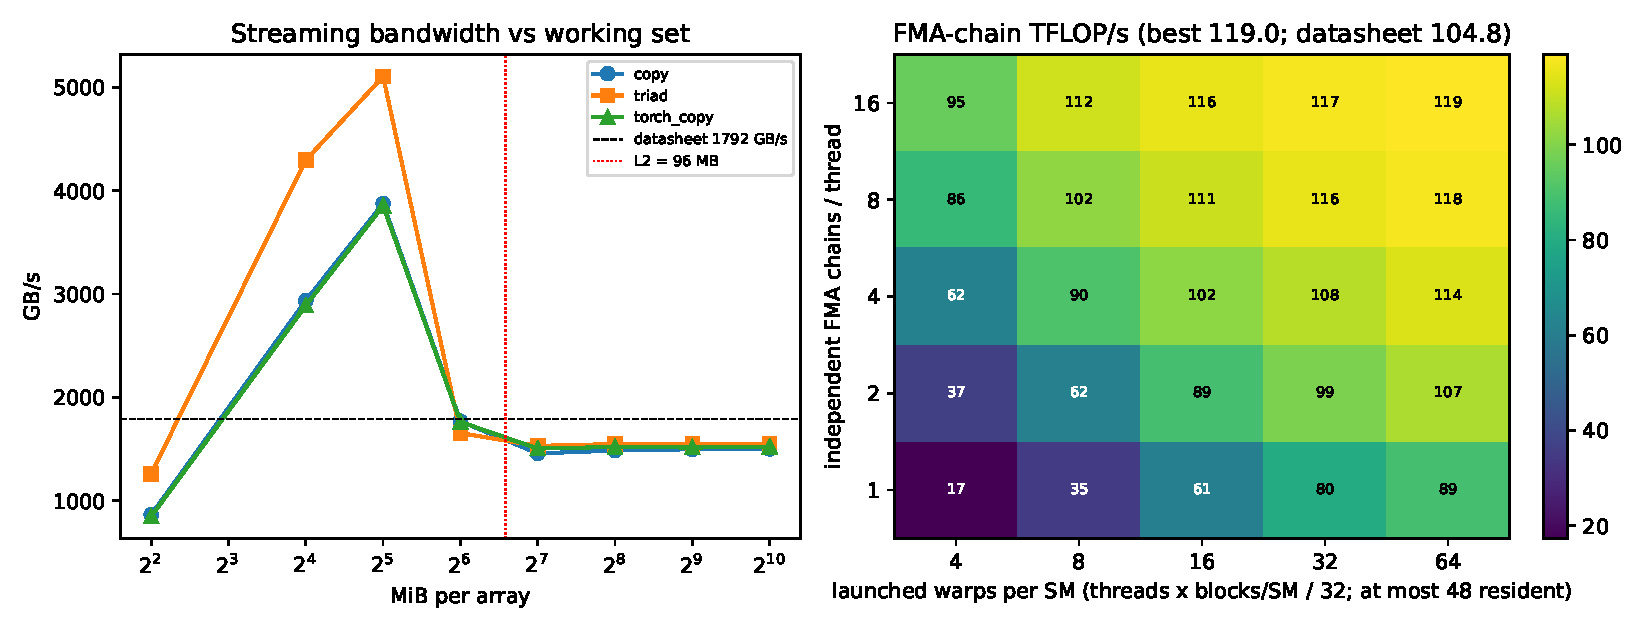
\includegraphics[width=\linewidth]{gpu_micro.pdf}
\caption{左：copy/triad/torch copy 带宽随每数组工作集大小，红线为 96~MB L2；右：FMA 链吞吐随独立链数与每 SM 启动 warp 数（每 SM 最多 48 个常驻）。数据：\texttt{micro\_bw.jsonl}、\texttt{micro\_fma.jsonl}。}
\label{fig:micro}
\end{figure}
\Cref{fig:micro} 左图有一道清楚的悬崖，位置正好是 L2 的容量。每数组 32~MiB（triad 总工作集 96~MiB）时，triad 达到 5107~GB/s；从 64~MiB 起掉到 1654~GB/s；
$\ge$256~MiB 后稳定在 1540--1549~GB/s，是规格 1792~GB/s 的 86\%。4~MiB 时只有 1256~GB/s，因为数据太少，kernel 启动开销（约 10~µs 量级）占了主导。
右图说明，要跑到 fp32 峰值，光有线程不够，还需要\emph{指令级并行}（ILP，同一线程里互不依赖、可以连续发射的指令）。
单条链、每 SM 一个 256 线程 block 时只有 34.9~TFLOP/s；16 条独立链时达到 118.97~TFLOP/s。
按 170~SM $\times$ 128 FMA/周期 $\times$ 2 FLOP 反推，有效时钟约 2.73~GHz，高于规格表 104.8~TFLOP/s 对应的 2.41~GHz boost。
tensor core 方面，cuBLAS 在 16384$^3$ 上 bf16 为 232.0、fp16 为 217.7、tf32 为 117.7~TFLOP/s。

\begin{findingbox}[：RTX 5090 的两个 ridge]
fp32：118.97/1.549 = 76.8~FLOP/B；bf16 tensor core：232.0/1.549 = 149.8~FLOP/B。数据常驻 L2 时，fp32 ridge 降到 118.97/5.107 = 23.3~FLOP/B。
\end{findingbox}

\subsection{SGEMM 优化阶梯}
\label{sec:ladder}
有了屋顶，就可以一级一级地看 SGEMM 怎样往上爬，以及每一级到底改掉了什么瓶颈。
\begin{figure}[H]
\centering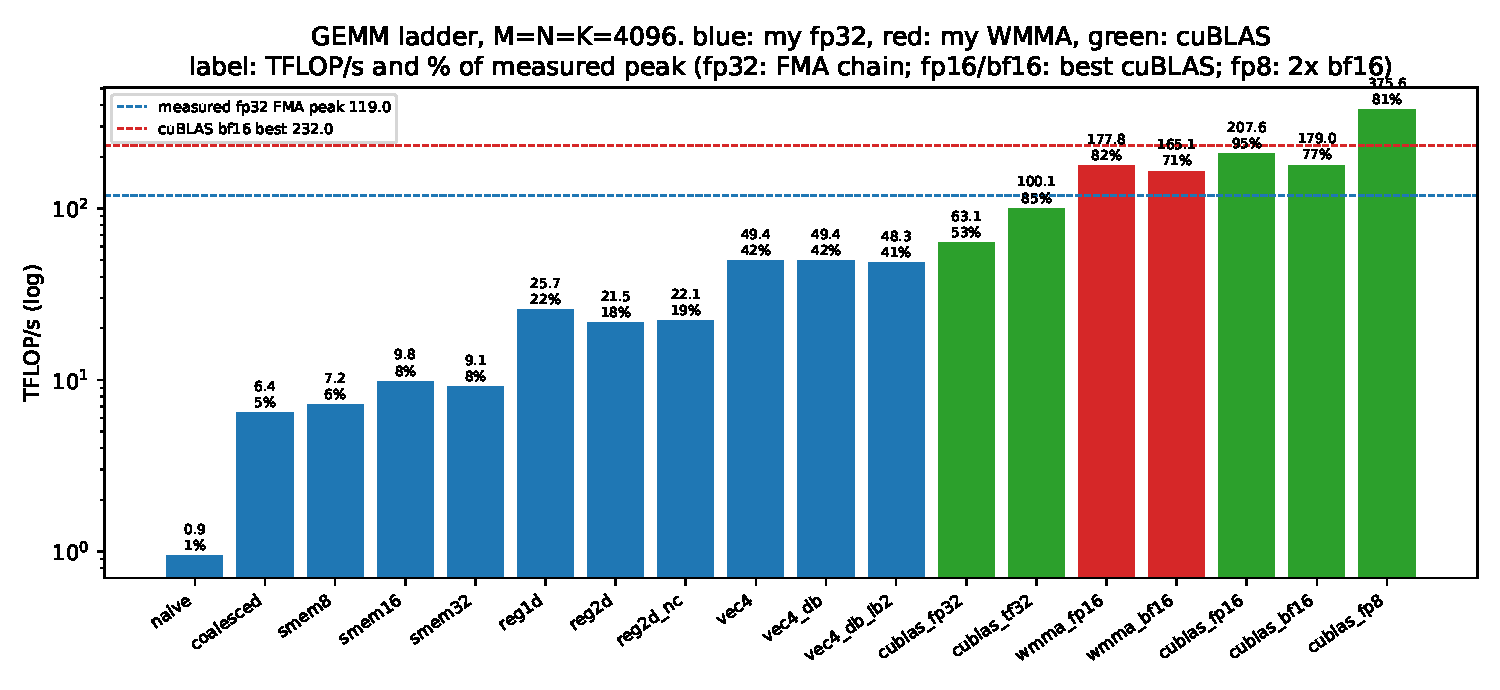
\includegraphics[width=\linewidth]{gpu_sgemm_ladder.pdf}
\caption{M=N=K=4096 的 GEMM 阶梯，标签为 TFLOP/s 与占对应实测峰值的比例。数据：\texttt{gemm\_ladder.jsonl}。}
\label{fig:ladder}
\end{figure}

\begin{table}[H]
\centering\small
\begin{tabular}{lrrrr}
\toprule
kernel & TFLOP/s & 占 fp32 峰值 & 相对上一级 & 误差 \\
\midrule
naive & 0.94 & 0.8\% & — & 2.85e-6 \\
coalesced & 6.43 & 5.4\% & 6.8$\times$ & 2.85e-6 \\
smem16 & 9.82 & 8.3\% & 1.53$\times$ & 2.85e-6 \\
reg1d & 25.73 & 21.6\% & 2.62$\times$ & 2.85e-6 \\
reg2d & 21.53 & 18.1\% & 0.84$\times$ & 2.85e-6 \\
reg2d\_nc & 22.07 & 18.6\% & 1.03$\times$ & 2.85e-6 \\
vec4 & 49.40 & 41.5\% & 2.24$\times$ & 2.85e-6 \\
vec4\_db & 49.44 & 41.6\% & 1.00$\times$ & 2.85e-6 \\
cuBLAS fp32 & 63.06 & 53.0\% & — & 9.20e-7 \\
cuBLAS tf32 & 100.05 & — & — & 3.02e-4 \\
WMMA fp16 / bf16（本文） & 177.80 / 165.11 & — & — & 6.07e-6 / 5.75e-6 \\
cuBLAS fp16 / bf16 & 207.57 / 178.99 & — & — & 3.62e-4 / 2.87e-3 \\
cuBLAS fp8 e4m3（\texttt{\_scaled\_mm}） & 375.57 & — & — & 2.85e-3 \\
\bottomrule
\end{tabular}
\caption{4096$^3$ 的阶梯（“相对上一级”按表中顺序）。reg2d\_nc 对比 reg2d，vec4 对比 reg2d\_nc。}
\label{tab:ladder}
\end{table}

下面逐级解释\cref{fig:ladder} 和\cref{tab:ladder}：
\begin{enumerate}
  \item naive 到 coalesced，快了 6.8 倍，只是交换了线程到行、列的映射。naive 中一个 warp 的 32 次 A 读落在 32 个不同的 128~B 行上，每条加载指令要取 32 个 sector；
        coalesced 中 B 的读是连续的、A 的读是广播，每条指令只要 4 个 sector。
  \item coalesced 到 smem，只快了 1.5 倍。显式复用让模型强度从 0.25 升到 3.99~FLOP/B，可提升不大，原因有两个：coalesced 版本已经借 L1/L2 隐式复用了大量数据；
        而 smem 版本每个 FMA 要做两次 shared 读，被 shared-memory 带宽卡住了。smem32 比 smem16 还慢（9.12 对 9.82），因为它每 block 1024 线程，理论 occupancy 只有 67\%（\cref{fig:kinfo}）。
  \item smem 到 reg1d，快了 2.6 倍。每个线程有 8 个累加器，一次 B 的 shared 读可以服务 8 个 FMA，每个 FMA 摊到的 shared 访问从 2 次降到 1.125 次。
  \item reg1d 到 reg2d 反而变慢（0.84 倍），这是最反直觉的一步。2D 分块的 FMA 与 shared 读之比更高（64 FMA 对 16 次读），按理应该更快。
        解析模型（\cref{fig:kinfo} 右）显示 B 读有 4-way、A 的转置写有 8-way bank conflict，而且每线程 110 个寄存器把 occupancy 压到了 33\%。
        可是消除冲突的 reg2d\_nc 只快了 2.5\%，说明冲突并不是主因。
  \item reg2d 到 vec4，快了 2.24 倍，是阶梯中第二大的单步提升。改动是换成 float4 全局读和 LDS.128 shared 读，每个 k 步每线程的 shared 加载\emph{指令}从 16 条降到 4 条，
        省下的指令发射槽留给了 FMA。这也回答了上一步的疑问：reg2d 真正的瓶颈是加载指令太多。
  \item vec4 到 vec4\_db 持平。BK=8 时每个 k 步只有 64 条 FMA，两级 smem 能省的同步本来就不多；而两级缓冲又把静态 smem 从 8~KiB 翻到 16~KiB，寄存器从 119 增到 128。
        这里还踩过一个坑：第一次编译时 vec4\_db 用了 129 个寄存器，$256\times129>32768$，每 SM 只能放 1 个 block，跑出 46.68~TFLOP/s，比 vec4 慢 6.6\%（\texttt{log\_campaign.txt}、\texttt{log\_wave2.txt}）。
        修改模板签名后 ptxas 分到 128 个寄存器，每 SM 回到 2 个 block，跑出 49.44（\texttt{ptxas\_sgemm.txt}、\texttt{kernel\_info.jsonl}）。
  \item 与 cuBLAS 相比，vec4 是 cuBLAS fp32 的 78.3\%。剩下的差距来自 warp 级分块、更深的流水和 SASS 级调度；如果允许 TF32，cuBLAS 还能再快 1.59 倍。
\end{enumerate}

4096$^3$ 只是一个点。换个规模，排名会不会变？
\begin{figure}[H]
\centering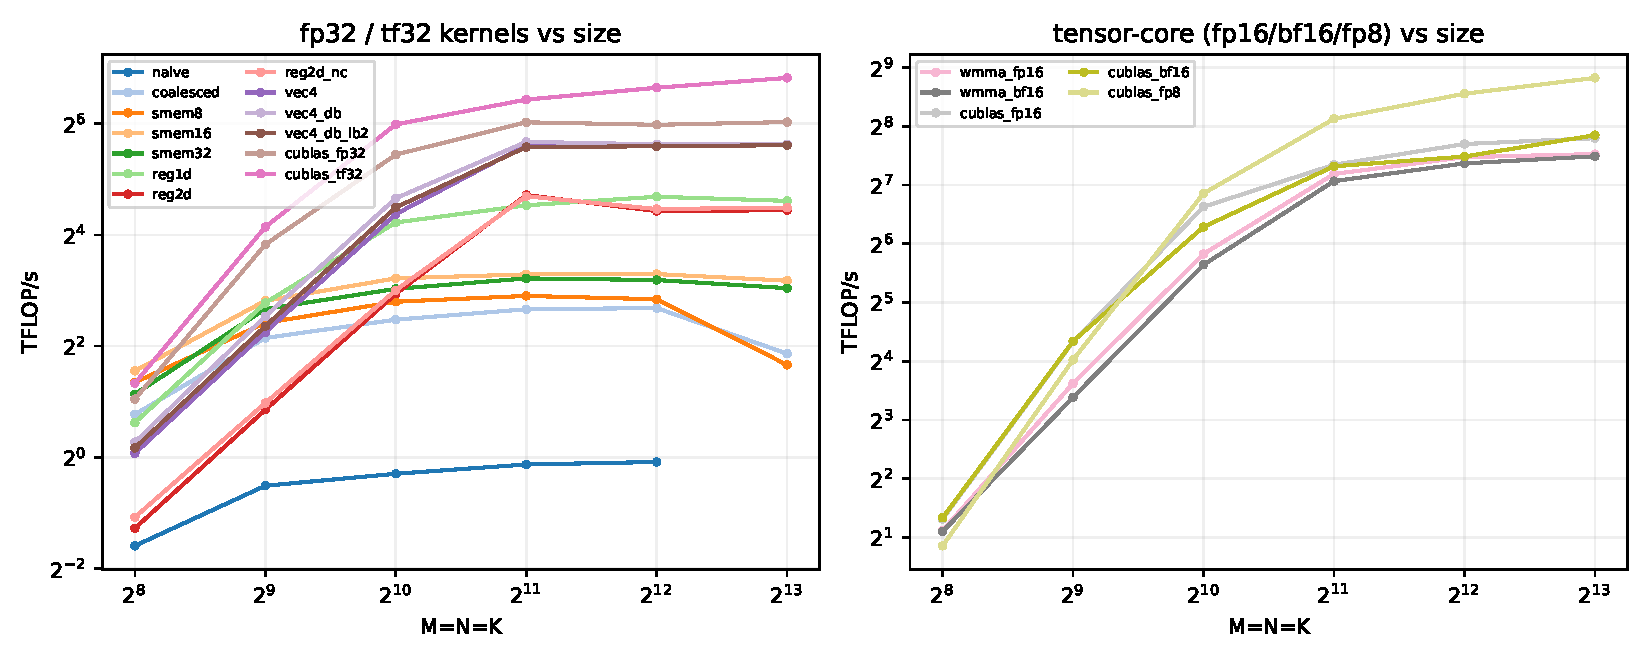
\includegraphics[width=\linewidth]{gpu_sgemm_sweep.pdf}
\caption{各 kernel 随方阵规模的吞吐（左 fp32/tf32，右 tensor core）。数据：\texttt{gemm\_ladder.jsonl}。}
\label{fig:sweep}
\end{figure}
\Cref{fig:sweep} 里有三个现象。
第一个是小矩阵的 wave quantization（block 数太少，填不满所有 SM）。256$^3$ 时 128$\times$128 tile 只有 4 个 block，170 个 SM 只用上 4 个，vec4 只有 1.05~TFLOP/s；
反倒是 16$\times$16 tile（256 个 block）的 smem16 最快（2.94）。这与脉动阵列「矩阵太小、开销摊不薄」是同一个道理。
第二个是 L2 悬崖。coalesced 和 smem8 在 8192$^3$ 掉到 3.64 和 3.17~TFLOP/s（4096$^3$ 时为 6.43 和 7.17），因为 8192 的 A、B 各有 256~MiB，远超 96~MB 的 L2，
跨 block 的复用不能再靠 L2 兜底。大 tile 的 kernel（reg1d、vec4）在两个规模上几乎持平，因为它们本来就不依赖 L2。
第三个是 tensor core 需要规模：WMMA fp16 在 1024$^3$ 只有 56.73，到 8192$^3$ 达到 184.36~TFLOP/s。

\subsection{tile 大小与算术强度}
CPU 模型说强度约等于 $t/b$。把同一个公式用到 GPU 的 fp32 上，能不能解释阶梯里的数字？
\begin{figure}[H]
\centering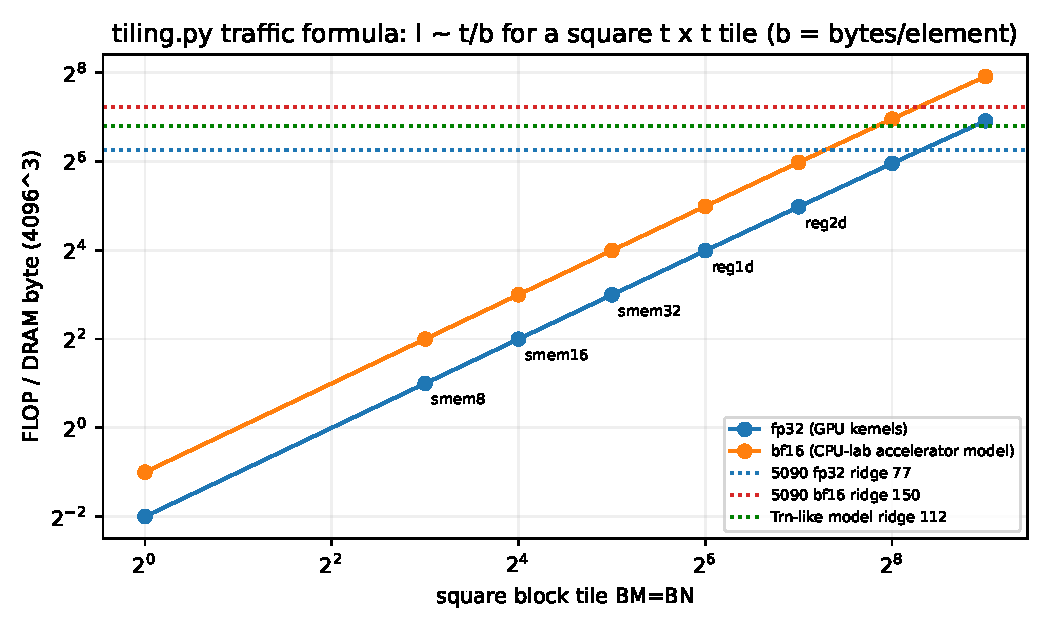
\includegraphics[width=0.85\linewidth]{gpu_intensity_model.pdf}
\caption{同一个流量公式（\texttt{tiling.py} 的 \texttt{tile\_stats}）在 fp32（GPU）与 bf16（CPU 侧加速器模型）下的强度，并标出各 ridge。}
\label{fig:imodel}
\end{figure}
\Cref{fig:imodel} 直接调用 CPU 侧的 \texttt{tile\_stats}。fp32 下 128 tile 的强度是 31.51~FLOP/B，正好是 bf16 下 63.02 的一半（$t/b$）。
对照 ridge 来看：在 Trainium 模型里，bf16 的 256 tile（124.12）已经越过了 ridge 111.9；而 RTX 5090 的 fp32 ridge 是 76.8，128 tile 只有 31.51，按 DRAM 模型仍是带宽受限。
可 vec4 实际跑到了 49.40~TFLOP/s，高于模型屋顶 $31.51\times1.549=48.8$。这只能说明实际的 DRAM 字节比模型少，也就是 L2 吸收了跨 block 的复用。

模型说 tile 越大强度越高，下一个问题自然是：那 tile 是不是越大越快？
\begin{figure}[H]
\centering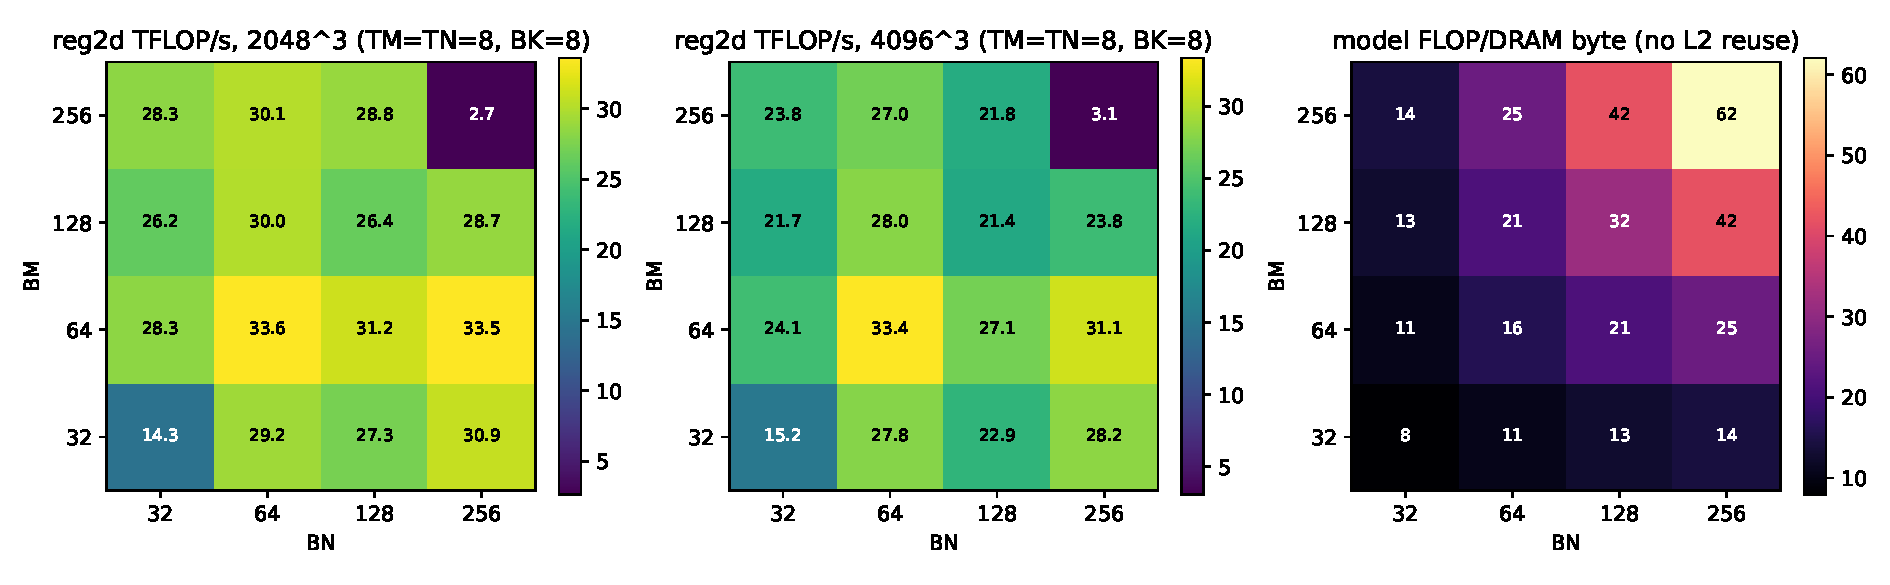
\includegraphics[width=\linewidth]{gpu_tile_heatmap.pdf}
\caption{reg2d（TM=TN=8，BK=8）在不同块 tile 下的吞吐（2048$^3$、4096$^3$）与模型强度。数据：\texttt{gemm\_tiles.jsonl}。}
\label{fig:heat}
\end{figure}
\Cref{fig:heat} 是作业里「调 tile 大小」问题的 GPU 版本，答案是否定的。模型强度沿对角线单调增加，从 32$\times$32 的 8.0 到 256$\times$256 的 62.1~FLOP/B，但吞吐并不跟着涨：
4096$^3$ 下 64$\times$64 最快（33.36~TFLOP/s），256$\times$256 只有 3.09。原因是 256$\times$256 每个 block 有 1024 线程，\texttt{\_\_launch\_bounds\_\_(1024)} 把寄存器压到 64 个，
可每个线程光累加器就要 64 个，于是 ptxas 报告了 1108 字节的 spill（寄存器放不下、溢出到本地内存，见 \texttt{ptxas\_sgemm.txt}）。
另一头，32$\times$32 每个 block 只有 16 个线程（半个 warp），同样很慢（15.18）。
可见 GPU 上的 tile 大小同时受三种片上容量约束：shared memory、寄存器文件和每 block 线程数，强度最高的点往往不是最快的点。这与 CPU 模型里「PSUM 容量封顶」是同一类约束。

\subsection{Occupancy 与 bank conflict（ncu 的替代）}
阶梯里有两个解释用到了 occupancy 和 bank conflict。由于没有 ncu，这里用 occupancy API 和解析模型把它们补上。
\begin{figure}[H]
\centering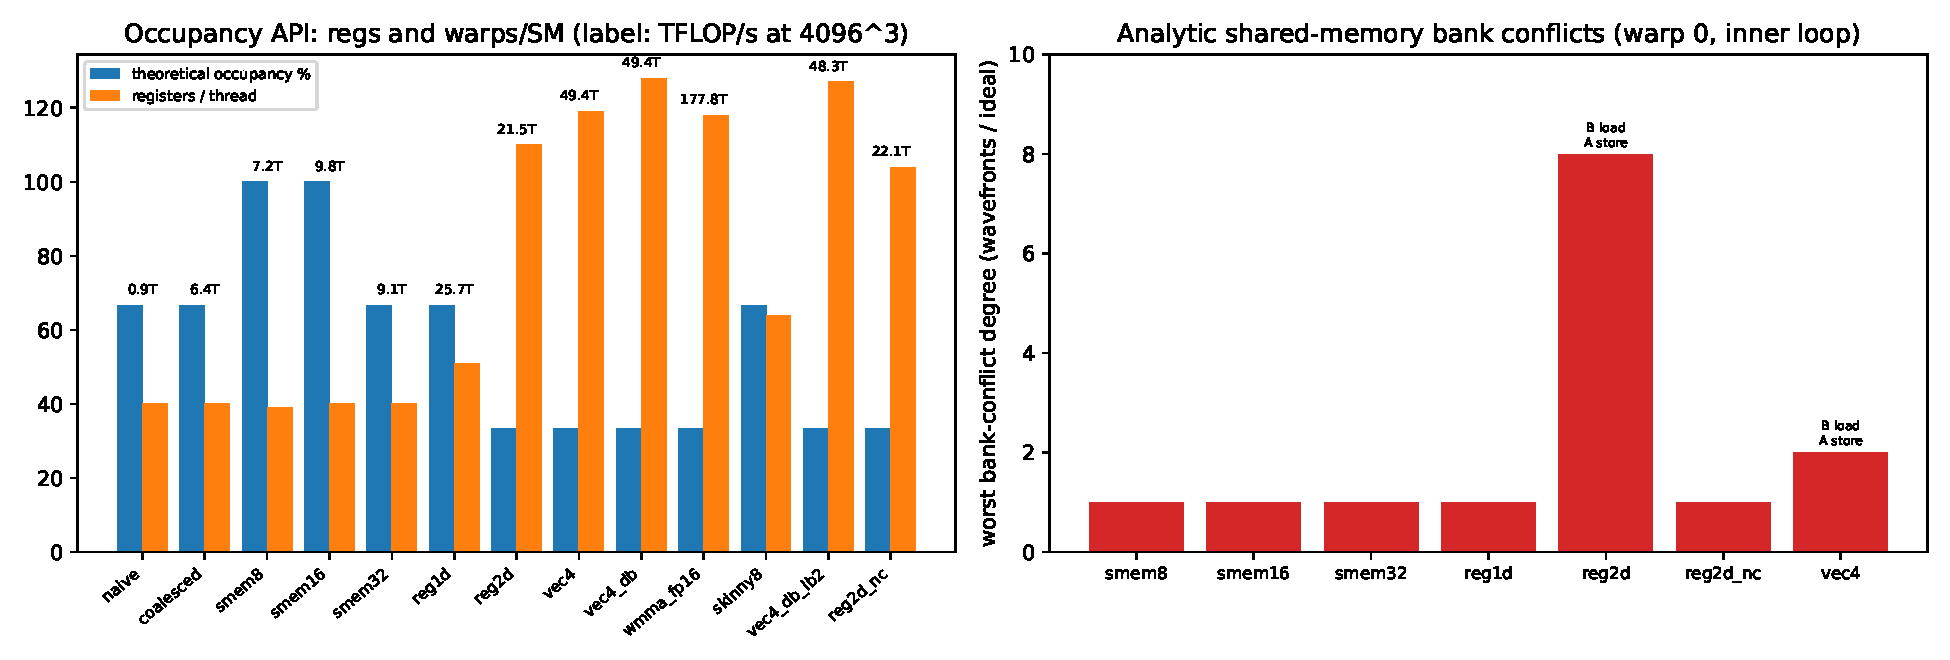
\includegraphics[width=\linewidth]{gpu_kernel_info.pdf}
\caption{左：CUDA occupancy API 给出的理论 occupancy 与每线程寄存器（标签为 4096$^3$ 吞吐）；右：解析 bank 模型给出的最坏冲突度。数据：\texttt{kernel\_info.jsonl}、\texttt{bank\_model.jsonl}。}
\label{fig:kinfo}
\end{figure}
\Cref{fig:kinfo} 左图里，occupancy 与性能是\emph{负相关}的：smem8/16 的理论 occupancy 是 100\%，却只有 7--10~TFLOP/s；vec4 和 WMMA 只有 33\%（每 SM 16 个 warp），却最快。
这正是 Volkov 的经典结论：用寄存器级的 ILP 换 occupancy~\cite{volkov2008,volkov2010}，每个线程多算一些，少几个 warp 也能把延迟藏住。
右图的解析模型假设 32 个 4 字节 bank，128 位访问按四分之一 warp 分相（phase）处理。按这个模型，reg2d 的 B 读 \texttt{Bs[k*BN+tcol*8+j]} 中，tcol 为 0、4、8、12 的线程落在同一个 bank，是 4-way；
A 的转置写 \texttt{As[c*BM+r]} 在一个 warp 内有 8 个 c 值打到同一个 bank，是 8-way。reg2d\_nc 补 4 个 float 后全部降为 1；vec4 的 B 读与 A 转置写为 2-way。
要强调的是，由于 \texttt{ncu} 不可用，这些都是\emph{模型}值，不是计数器读数。

\subsection{GEMM 在 roofline 上的位置}
把各 kernel 画到实测 roofline 上，可以检验「L2 吸收了复用」这个解释到底站不站得住。
\begin{figure}[H]
\centering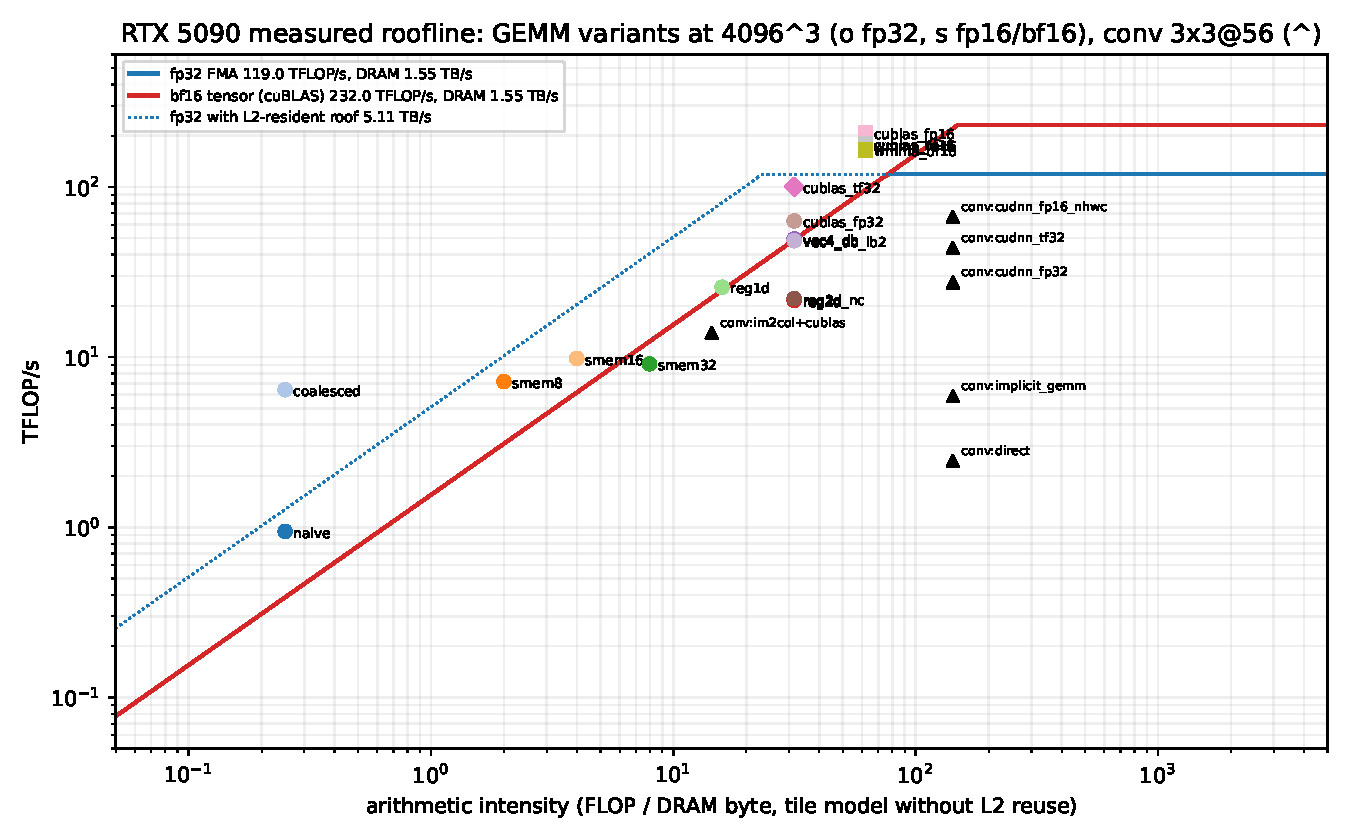
\includegraphics[width=\linewidth]{gpu_roofline.pdf}
\caption{实测 roofline：DRAM 1.549~TB/s、L2 5.107~TB/s、fp32 118.97、bf16 232.0~TFLOP/s。GEMM 点（4096$^3$）的横坐标用 tile 模型强度（无 L2 复用），卷积点为 3$\times$3@56 C64、batch 8，横坐标用 $x+w+y$（im2col 额外加两倍缓冲区）的强度。}
\label{fig:roof}
\end{figure}
按 DRAM 模型，smem8/16/32 和 reg1d 都应该落在\cref{fig:roof} 的 DRAM 斜线以下。实际上 coalesced、smem8 等明显\emph{高于}这条斜线，例如 smem8 在 2.0~FLOP/B 处跑出 7.17~TFLOP/s，
而斜线在这里只有 3.10；它们更接近 L2 斜线，因为 4096$^3$ 的 A+B=128~MiB 有相当一部分留在了 L2 里。
到了 8192$^3$，L2 帮不上忙，smem8 跑出 3.17~TFLOP/s，按 \cref{eq:traffic} 反推的 DRAM 带宽是 1585~GB/s，与 triad 的 1549~GB/s 只差 2.3\%。
\textbf{这是本文最重要的交叉验证：只要工作集超过 L2，CPU 部分的 scratchpad 流量模型在 GPU 上定量成立。}
tensor-core 的点（WMMA、cuBLAS fp16/bf16）位于 62.06~FLOP/B，低于 bf16 ridge 149.8，却跑到 165--208~TFLOP/s，同样说明 L2 吸收了复用。
卷积的 cuDNN 点在 146~FLOP/B 处只有 27.4（fp32）到 66.4（fp16）~TFLOP/s。限制它的不是带宽，而是 batch 8 的层太小，受启动、尾部效应和 SM 利用率的影响。

\subsection{精度与速度}
阶梯表里的误差一栏差了好几个数量级。比较低精度 kernel 之前，得先弄清这些误差从哪里来。
\begin{figure}[H]
\centering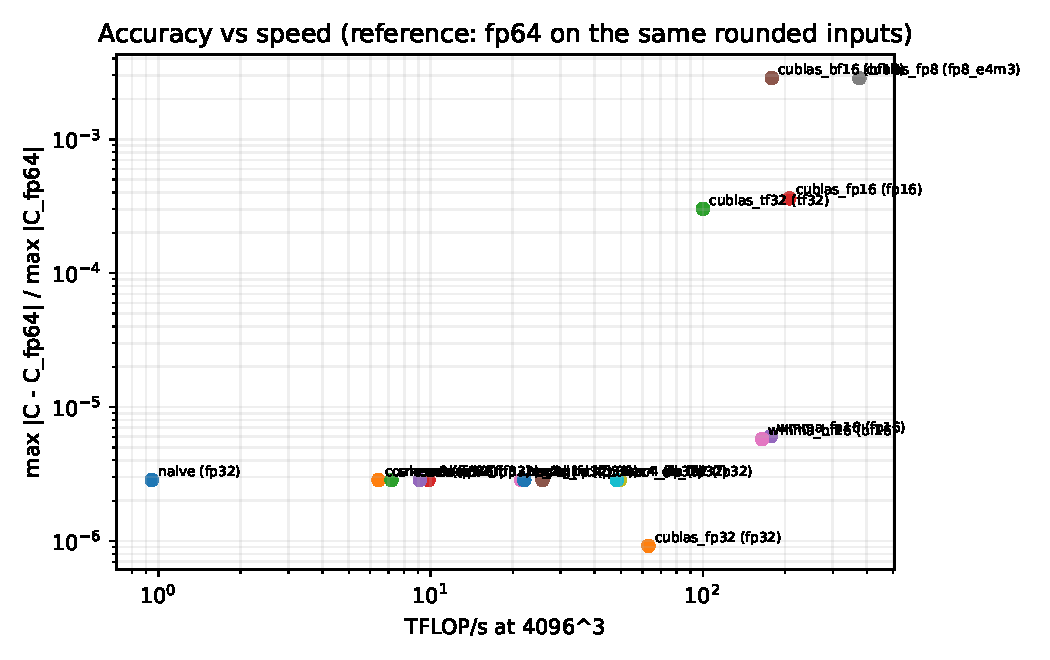
\includegraphics[width=0.82\linewidth]{gpu_precision.pdf}
\caption{4096$^3$ 各 kernel 的误差（相对 fp64，在同一组已舍入输入上）与吞吐。数据：\texttt{gemm\_ladder.jsonl}。}
\label{fig:prec}
\end{figure}
所有 fp32 kernel 的误差都是 2.85e-6，量级相同，因为累加顺序相近。cuBLAS fp32 为 9.20e-7，我推测是它的分块累加顺序让部分和更短，但没有验证。TF32 为 3.02e-4，对应 10 位尾数的乘法舍入。
更意外的是，cuBLAS fp16/bf16（3.62e-4 / 2.87e-3）比我的 WMMA（6.07e-6 / 5.75e-6）误差大两个数量级。这并不是它累加得更差：\texttt{torch.matmul} 把 C 输出成 fp16/bf16，
误差由输出舍入（bf16 的 $2^{-9}\approx2\times10^{-3}$）主导，而我的 kernel 输出的是 fp32。FP8 e4m3 的 2.85e-3 同样来自 bf16 输出舍入。
所以比较低精度 kernel 时，必须先说明输出精度，否则误差对比没有意义。

\subsection{Skinny GEMM（decode 形）}
LLM 推理的 decode 阶段，每步只处理很少几个 token，GEMM 的 $M$ 很小。这时问题从「算得够不够快」变成了「权重读得够不够快」。
\begin{figure}[H]
\centering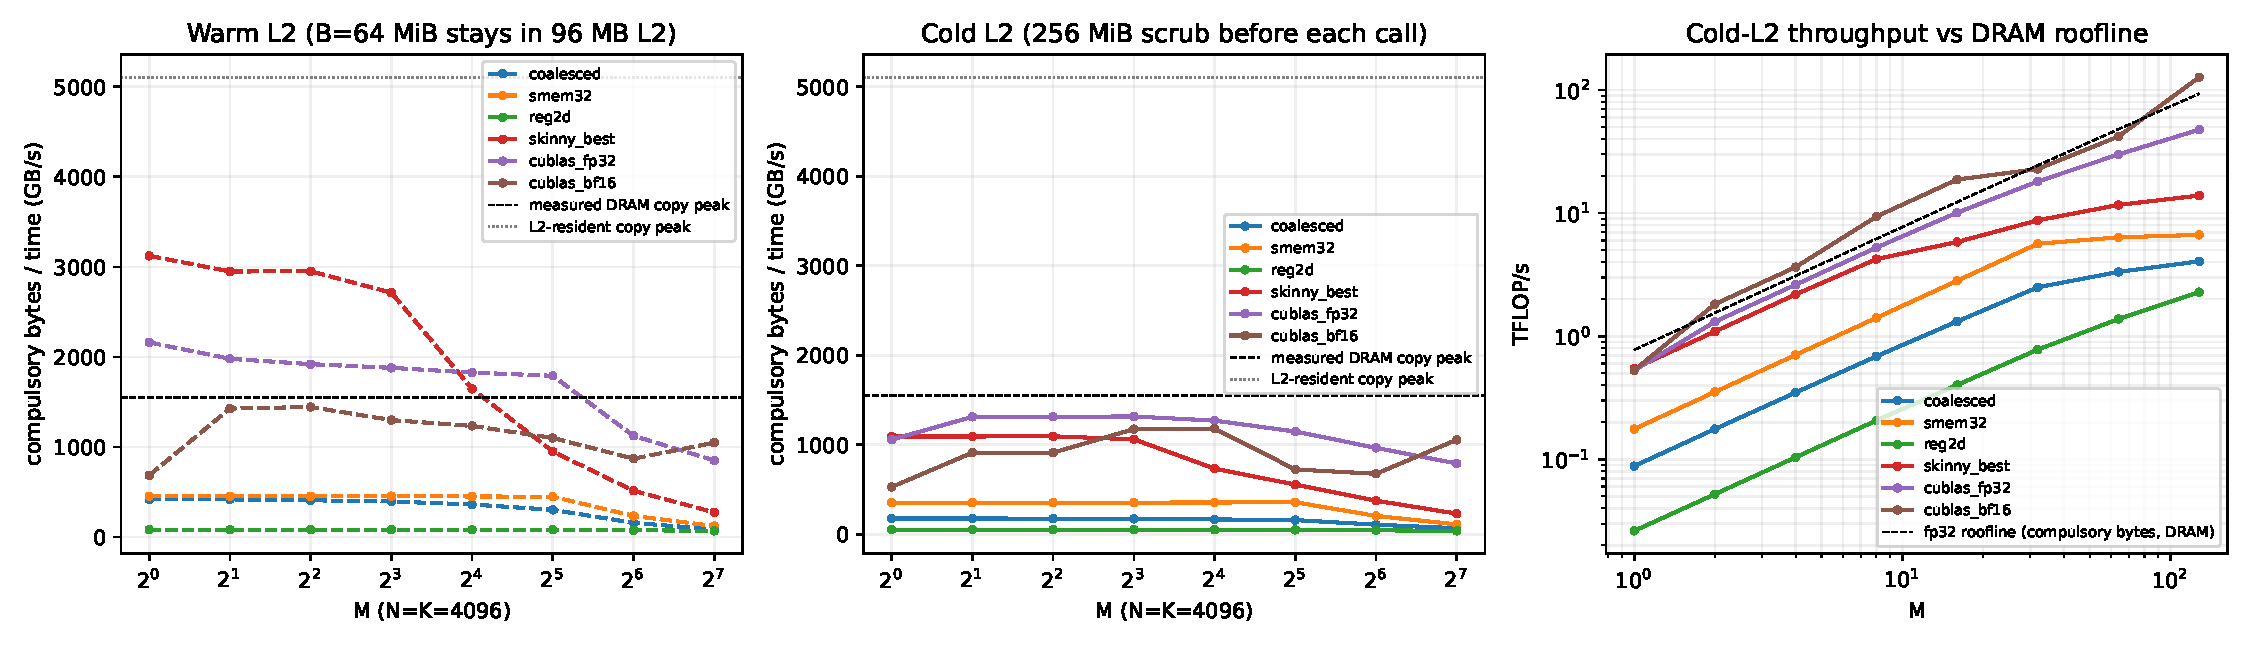
\includegraphics[width=\linewidth]{gpu_skinny.pdf}
\caption{N=K=4096，M=1..128。左：warm L2；中：每次调用前刷 256~MiB 的 cold L2；右：cold L2 的吞吐与 DRAM roofline。纵轴为“必需字节 / 时间”。数据：\texttt{gemm\_skinny.jsonl}。}
\label{fig:skinny}
\end{figure}
decode 阶段的 GEMM 强度约为 $2M/b$（$M\ll N,K$ 时），M=1 时 fp32 只有 0.5~FLOP/B，注定是带宽受限。
\Cref{fig:skinny} 左图里，我的 split-K kernel 在 M=1 时「跑出」了 3122~GB/s，超过了 DRAM 带宽。这是一个测量陷阱：B 只有 64~MiB，反复调用时一直留在 96~MB 的 L2 里。
中图把 L2 冲掉后，M=1 降到 1093~GB/s（DRAM 峰值的 70.6\%），与 cuBLAS fp32 的 1058~GB/s 持平；M=8 时 cuBLAS 为 1316，我的为 1061。
M=64 时 cuBLAS fp32 仍有 965~GB/s，我的 kernel 只剩 375，因为它每 8 行就重新读一遍 B，流量相当于放大了 8 倍（一部分被 L2 吸收）。
通用的 128$\times$128 tile 在 M=1 时浪费了 127/128 的计算行，cold 时只有 52~GB/s。

\begin{findingbox}[：小 batch 的 GEMM 看带宽，不看 FLOP]
M=1 时最好的 fp32 实现也只有 0.55~TFLOP/s（cold），不到 fp32 峰值的 0.5\%；bf16 把字节数减半，cuBLAS bf16 在 M=128 时（cold）有 127.1~TFLOP/s。
\end{findingbox}

\subsection{卷积：direct、im2col、implicit GEMM 与 cuDNN}
\label{sec:conv}
回到作业的第二部分：卷积改写成 GEMM 之后，几种写法在 GPU 上谁快谁慢？
\begin{figure}[H]
\centering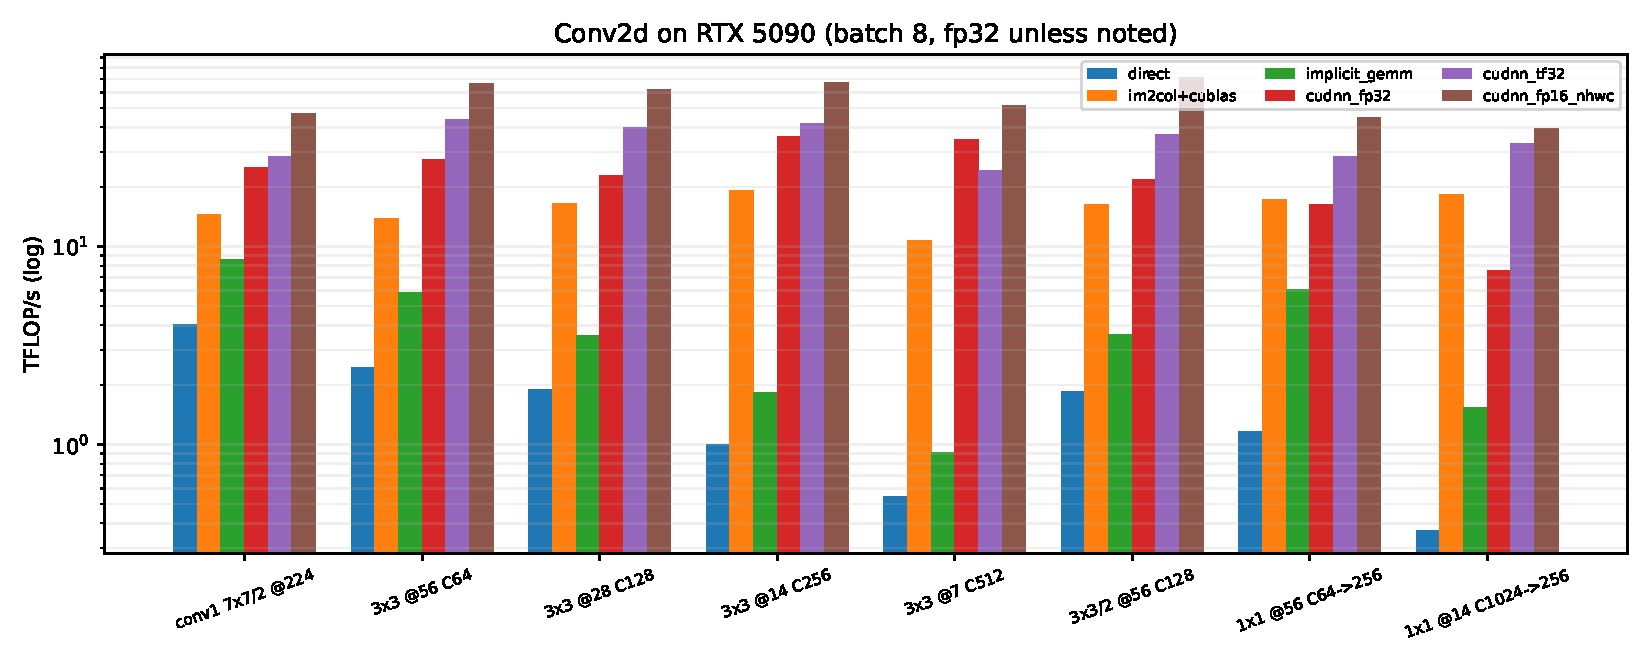
\includegraphics[width=\linewidth]{gpu_conv.pdf}
\caption{ResNet 类层（batch 8，fp32，cuDNN fp16 使用 NHWC）的吞吐。数据：\texttt{conv.jsonl}。}
\label{fig:conv}
\end{figure}
\begin{table}[H]
\centering\small
\begin{tabular}{lrrrrrr}
\toprule
层 & direct & im2col+cuBLAS & 膨胀 & implicit & cuDNN fp32 & cuDNN fp16 \\
\midrule
conv1 7$\times$7/2 @224 & 0.470 & 0.130 & 12.25 & 0.220 & 0.075 & 0.040 \\
3$\times$3 @56 C64 & 0.754 & 0.133 & 9.00 & 0.314 & 0.068 & 0.028 \\
3$\times$3 @28 C128 & 0.974 & 0.113 & 9.00 & 0.522 & 0.081 & 0.030 \\
3$\times$3 @14 C256 & 1.849 & 0.097 & 9.00 & 1.014 & 0.051 & 0.028 \\
3$\times$3 @7 C512 & 3.403 & 0.172 & 9.00 & 2.019 & 0.054 & 0.036 \\
3$\times$3/2 @56 C128 & 0.997 & 0.113 & 2.25 & 0.513 & 0.085 & 0.026 \\
1$\times$1 @56 C64$\to$256 & 0.707 & 0.047 & 1.00 & 0.136 & 0.050 & 0.018 \\
1$\times$1 @14 C1024$\to$256 & 2.237 & 0.045 & 1.00 & 0.534 & 0.109 & 0.021 \\
\bottomrule
\end{tabular}
\caption{卷积耗时（ms，batch 8）。我的 kernel 与 im2col+cuBLAS 的误差均 $\le 2.5\times10^{-6}$；cuDNN fp32 最大为 $1.7\times10^{-5}$（3$\times$3@7 C512），可能选用了非直接累加的算法。}
\label{tab:conv}
\end{table}
\Cref{tab:conv} 的结论和 CPU 端不一样，有三点值得说。
其一，我的 direct 和 implicit GEMM 都远慢于 im2col+cuBLAS，因为它们的「GEMM 部分」远不如 cuBLAS：implicit GEMM 的 gather 每个元素要做 6 次整数除法或取模，
而且没有 float4，也没有双缓冲。可见 implicit GEMM 的优势（不物化 im2col）只有在 GEMM 内核本身足够好时才能体现出来。
其二，channel 深、空间小的层（3$\times$3@7 C512、1$\times$1@14 C1024）上 direct 卷积最差：OW=7 时，一个 128 线程的 block 只有 7 个线程在干活。
其三，cuDNN fp32 在 1$\times$1@14 C1024 上（0.109~ms）反而比 im2col+cuBLAS（0.045~ms）慢，说明 cuDNN 的启发式选择并不总是最优。

im2col 的代价究竟花在哪里，下图把它拆开来看。
\begin{figure}[H]
\centering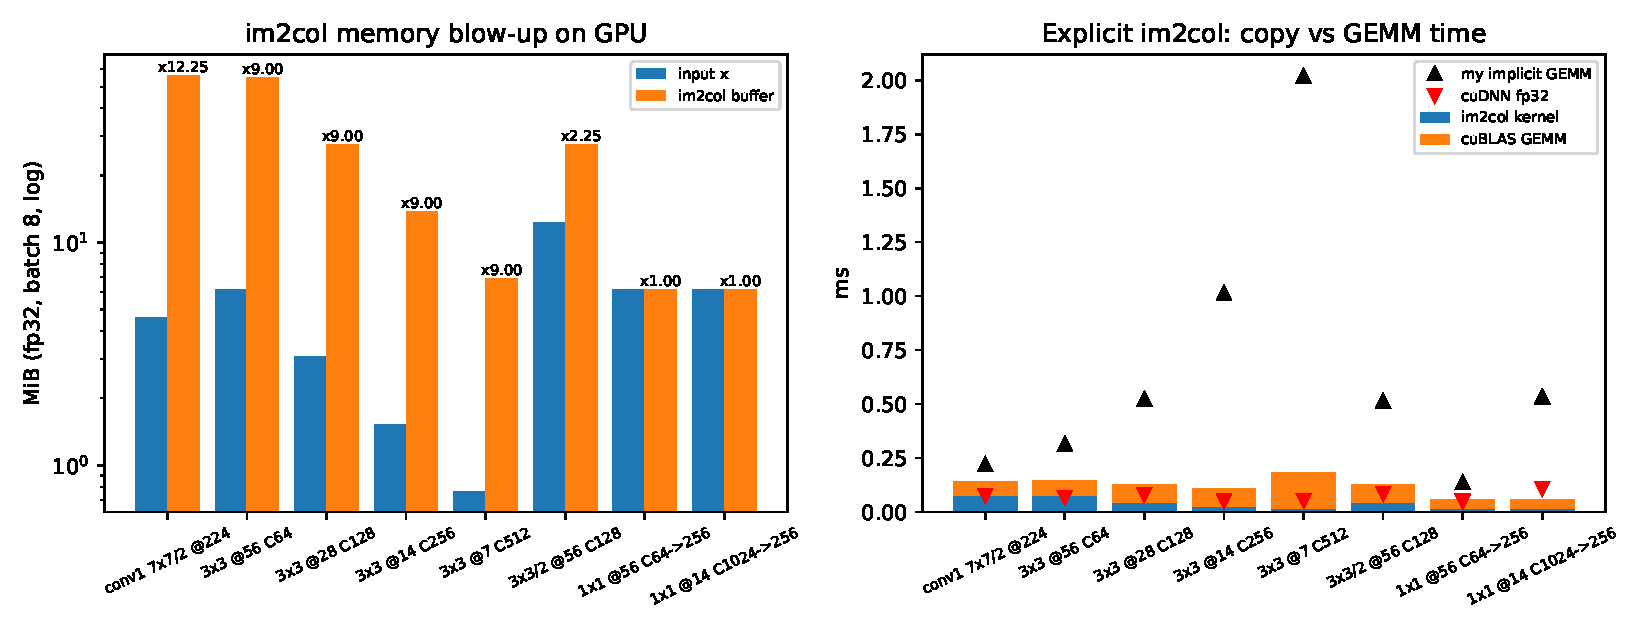
\includegraphics[width=\linewidth]{gpu_im2col.pdf}
\caption{左：im2col 缓冲区与输入大小（batch 8，log）；右：显式 im2col 的时间分解，对照我的 implicit GEMM 与 cuDNN。数据：\texttt{conv.jsonl}。}
\label{fig:im2colgpu}
\end{figure}
\Cref{fig:im2colgpu} 中，conv1 的 im2col 缓冲区有 56.3~MiB，是输入 4.59~MiB 的 12.25 倍；im2col kernel 用 0.077~ms，cuBLAS 用 0.064~ms，拷贝占了 55\%。
3$\times$3@56 C64 也有 53\% 的时间花在拷贝上。3$\times$3@7 C512 的缓冲区只有 6.9~MiB，拷贝只占 8\%，时间主要花在 GEMM（K=4608、N=392）上。
所以显式 im2col 的代价随膨胀倍数和空间分辨率增长；早期层（H 大、C 小）最贵，这正是 implicit GEMM 与 Winograd~\cite{lavin2016} 想要解决的场景。

\subsection{融合 conv + ReLU + maxpool}
最后是作业的第三部分：融合到底能省多少？先算账，再看实测。
\begin{figure}[H]
\centering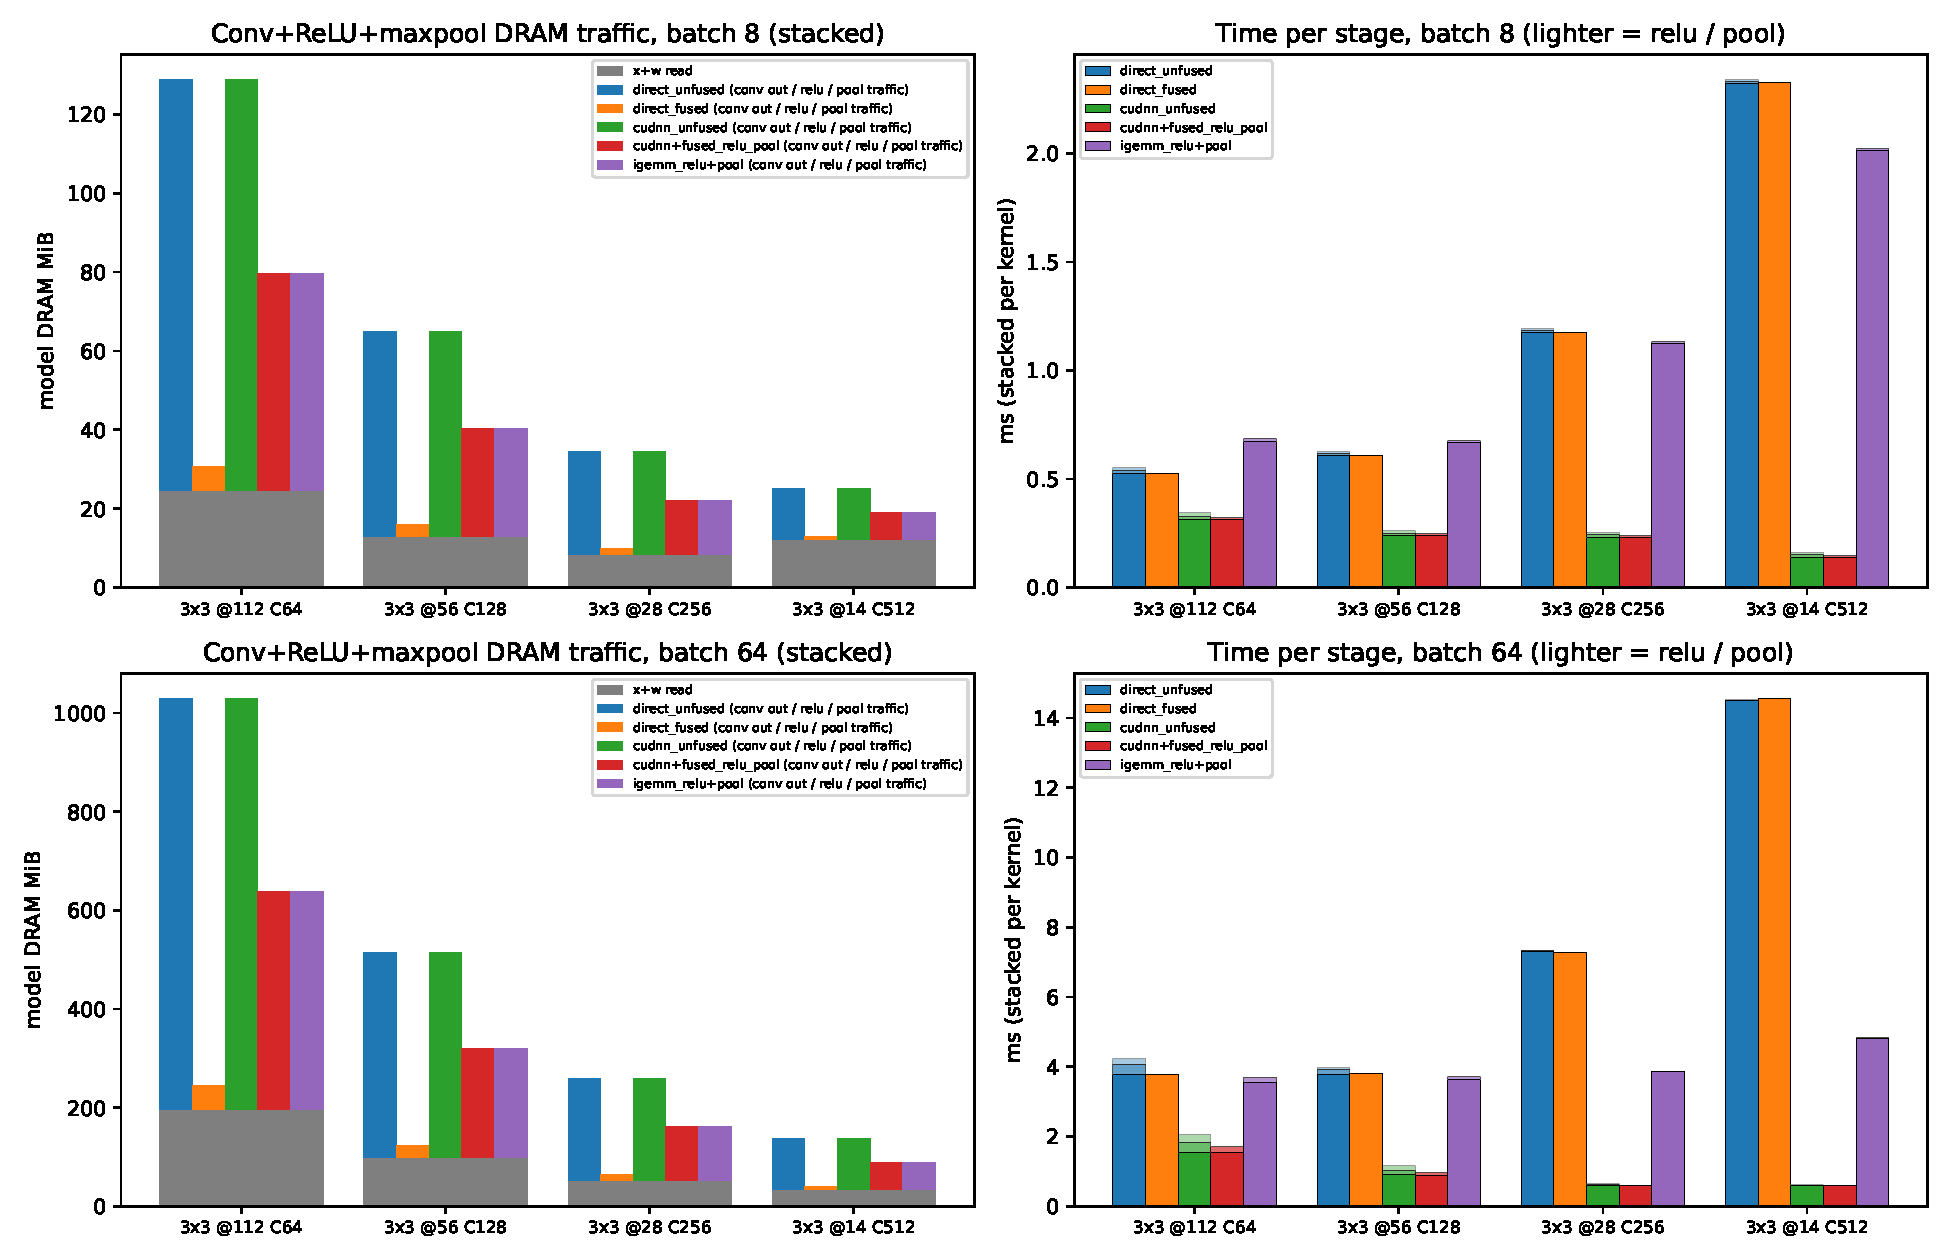
\includegraphics[width=\linewidth]{gpu_fusion.pdf}
\caption{VGG~\cite{simonyan2015} 类 3$\times$3 层的 conv+ReLU+maxpool：模型 DRAM 流量（左，灰色为 $x+w$ 的读，彩色为中间张量相关流量）与分阶段时间（右）。上：batch 8；下：batch 64。数据：\texttt{conv\_fusion.jsonl}。}
\label{fig:fusion}
\end{figure}
设卷积输出的字节数为 $Y$。非融合路径里，卷积写 $Y$，ReLU 读 $Y$ 写 $Y$，pool 读 $Y$ 写 $Y/4$，中间流量共 $4.25Y$；融合路径只写 $Y/4$。
如果只融合 ReLU+pool（放在 cuDNN 卷积之后），流量是 $Y+Y+Y/4=2.25Y$。
\begin{table}[H]
\centering\footnotesize
\begin{tabular}{llp{4.6cm}rrr}
\toprule
层 & batch & 方法 & 模型 DRAM MiB & 时间 ms & 省下 µs \\
\midrule
3$\times$3 @112 C64 & 64 & direct 非融合 $\to$ 融合 & 1029.1 $\to$ 245.1 & 4.230 $\to$ 3.768 & 462 \\
3$\times$3 @112 C64 & 64 & cuDNN+ReLU+pool $\to$ cuDNN+融合 ReLU-pool & 1029.1 $\to$ 637.1 & 2.062 $\to$ 1.711 & 351 \\
3$\times$3 @56 C128 & 64 & direct 非融合 $\to$ 融合 & 515.1 $\to$ 123.1 & 3.986 $\to$ 3.801 & 185 \\
3$\times$3 @56 C128 & 64 & cuDNN $\to$ cuDNN+融合 ReLU-pool & 515.1 $\to$ 319.1 & 1.155 $\to$ 0.961 & 194 \\
3$\times$3 @14 C512 & 64 & direct 非融合 $\to$ 融合 & 137.6 $\to$ 39.6 & 14.523 $\to$ 14.552 & $-$30 \\
3$\times$3 @112 C64 & 8 & direct 非融合 $\to$ 融合 & 128.8 $\to$ 30.8 & 0.551 $\to$ 0.526 & 26 \\
3$\times$3 @56 C128 & 8 & direct 非融合 $\to$ 融合 & 64.9 $\to$ 15.9 & 0.627 $\to$ 0.609 & 17 \\
\bottomrule
\end{tabular}
\caption{融合的流量与时间（“时间”为各阶段中位数之和）。}
\label{tab:fusion}
\end{table}

\begin{figure}[H]
\centering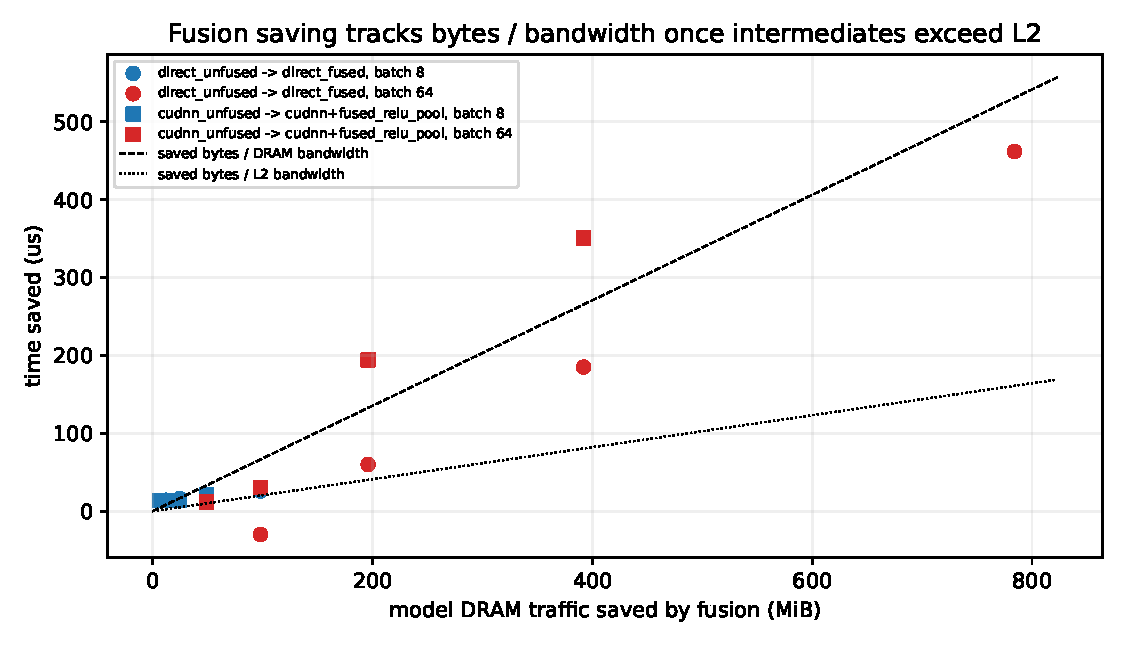
\includegraphics[width=0.8\linewidth]{gpu_fusion_saving.pdf}
\caption{融合省下的时间 vs 省下的模型 DRAM 字节；虚线为按 DRAM 带宽换算，点线为按 L2 带宽换算。}
\label{fig:fsave}
\end{figure}
\Cref{fig:fusion,fig:fsave,tab:fusion} 给出了官方 A4 融合问题的定量答案。同一个融合，收益差别很大，关键看中间张量落在哪里：
\begin{itemize}
  \item batch 64、3$\times$3@112 C64：卷积输出 $Y$=196~MiB，中间张量远超 L2。非融合的 ReLU kernel 用 0.290~ms 处理 $2Y$（411~MB），即 1.42~TB/s；pool 用 0.163~ms 处理 $1.25Y$，即 1.58~TB/s，
        两者都贴着 DRAM 屋顶。融合把这 0.453~ms 的纯搬运几乎全部省掉了（实测省 462~µs）。
  \item batch 8：中间张量 $\le$26~MB，留在 L2 里，ReLU 和 pool 各自只要 10--15~µs，融合只省 17--26~µs。在\cref{fig:fsave} 中，这些蓝点贴着 L2 点线。
  \item 3$\times$3@14 C512：卷积本身就要 14.5~ms（计算受限，而且我的 direct kernel 很慢），中间张量只有 25.7~MB，融合的收益淹没在噪声里（$-$30~µs）。
\end{itemize}
换句话说，融合的收益约等于「省下的字节」除以「这些字节原本所在那一级存储的带宽」。Trainium 上 SBUF 外面直接就是 HBM，没有 96~MB 的 L2 兜底，所以官方作业里的融合收益更接近本文 batch 64 的情形。

\begin{findingbox}[：融合省的是“中间张量的往返”，收益取决于它落在哪一级存储]
同一个融合，在中间张量溢出 L2 时省 0.46~ms（11\%），在 L2 内只省 17~µs（3\%），在计算受限的层上为零。
\end{findingbox}

\subsection{第三张卡：RTX 6000D 的算力不是一个稳定的数}\label{sec:6000d}

做跨卡比较时，RTX 6000D 的数字对不上：它的 FlashAttention 只有 5090 的 0.43 倍，cuBLAS fp16 8192$^3$ 是 0.64 倍，而 \texttt{peaks.json} 里的 bf16 峰值却是 0.97 倍。
这几个数不可能同时代表它的算力。我用两个探针来判断哪个数是真的。

第一个探针是持续负载（\texttt{gpu/sustained\_probe.py}）：每个形状连续跑 8~s，每 0.25~s 一个窗口，同时以 100~ms 间隔采 nvidia-smi。
每个形状从第一个窗口起就是平的，8192$^3$ 和 16384$^3$ 稳定在 141--145~TFLOP/s。SM 时钟 2422~MHz 纹丝不动，功耗最高 443~W（上限 600~W），没有任何降频原因，
所以既不是过热，也不是撞了功耗墙。

\begin{figure}[H]
\centering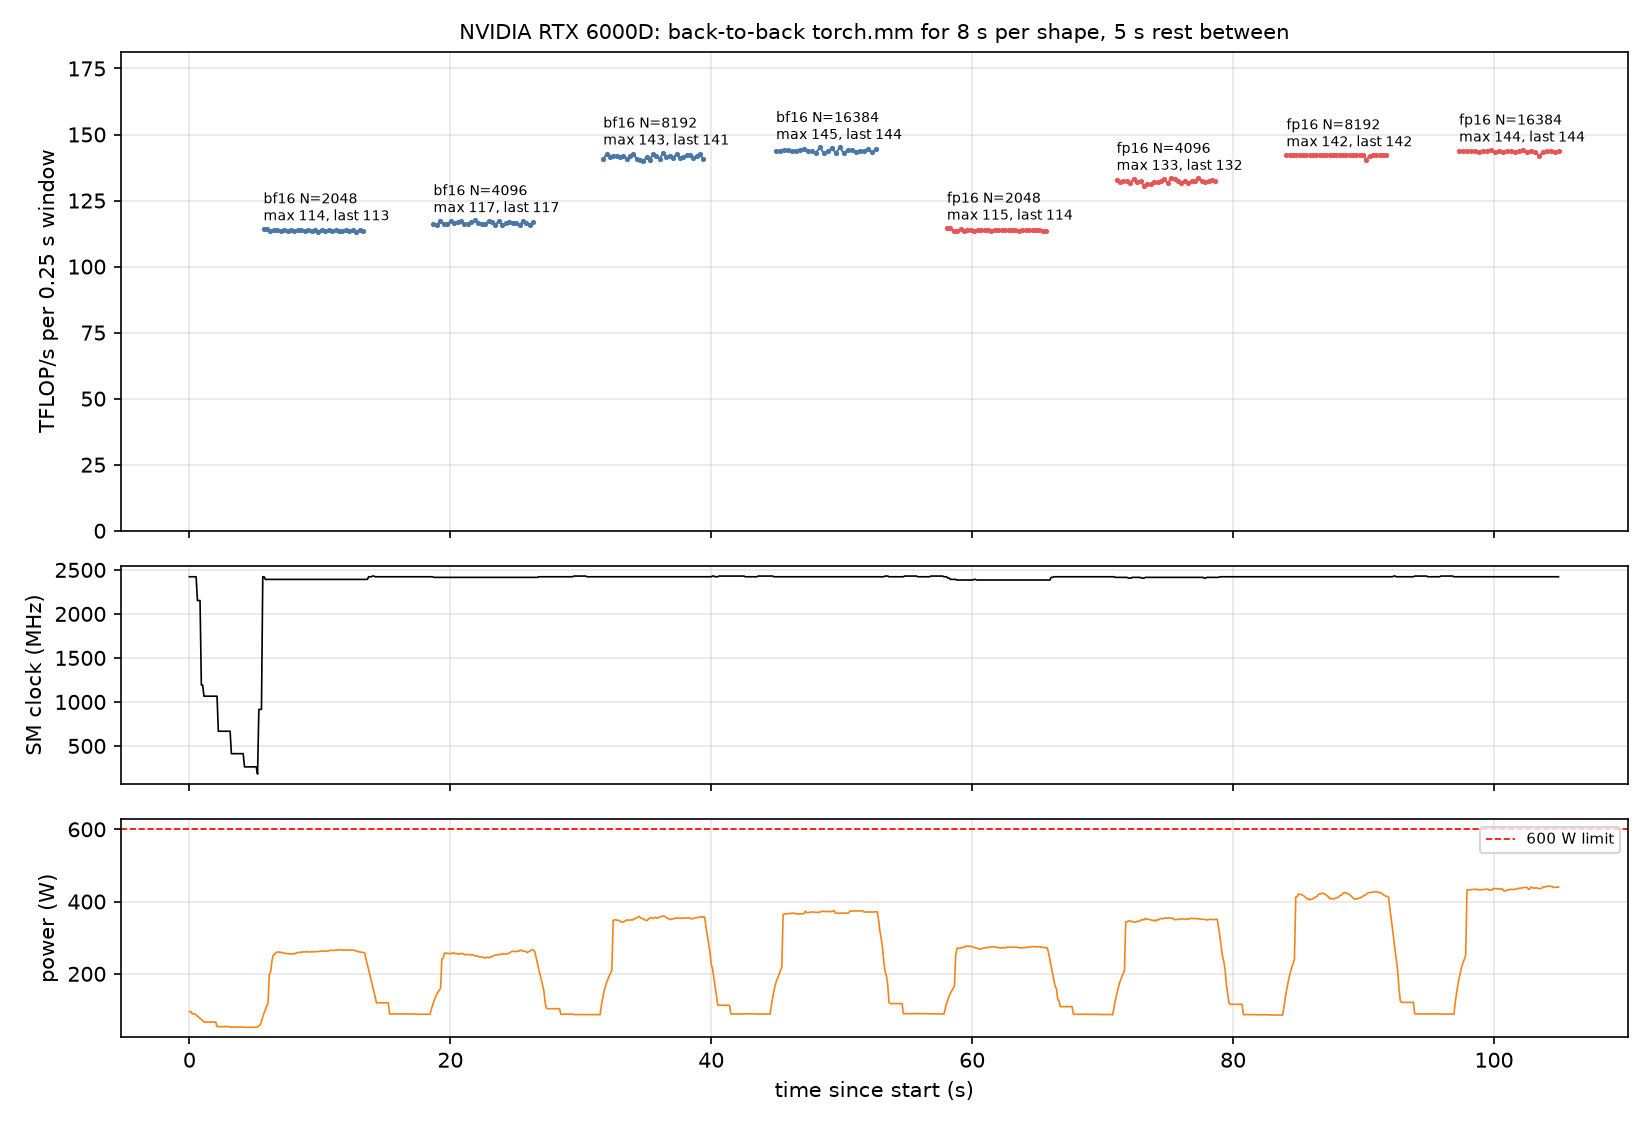
\includegraphics[width=\linewidth]{rtx6000d/sustained.png}
\caption{RTX 6000D 持续 8~s 的 matmul：每 0.25~s 窗口的 TFLOP/s、SM 时钟与功耗。}
\label{fig:sustained}
\end{figure}

第二个探针是逐 kernel 计时（\texttt{gpu/burst\_probe.py}）：每次 \texttt{torch.mm} 都用一对 CUDA event 单独计时。结果发现单个 kernel 的速度是双峰的。
2048$^3$ 有 58\% 的 kernel 落在 240--260~TFLOP/s，其余在 50--80；4096$^3$ 最快 303，中位数 136。快段和慢段交替出现，快段 0.15--0.75~ms，慢段 0.2--4.4~ms，没有固定周期；
kernel 之间平均只空 0.4~µs。我还扫了运行前的空闲时长，从 0~ms 到 3~s，整段平均都一样（bf16 116--118），所以这也不是「攒一段预算、用完就降速」的模型。

\begin{figure}[H]
\centering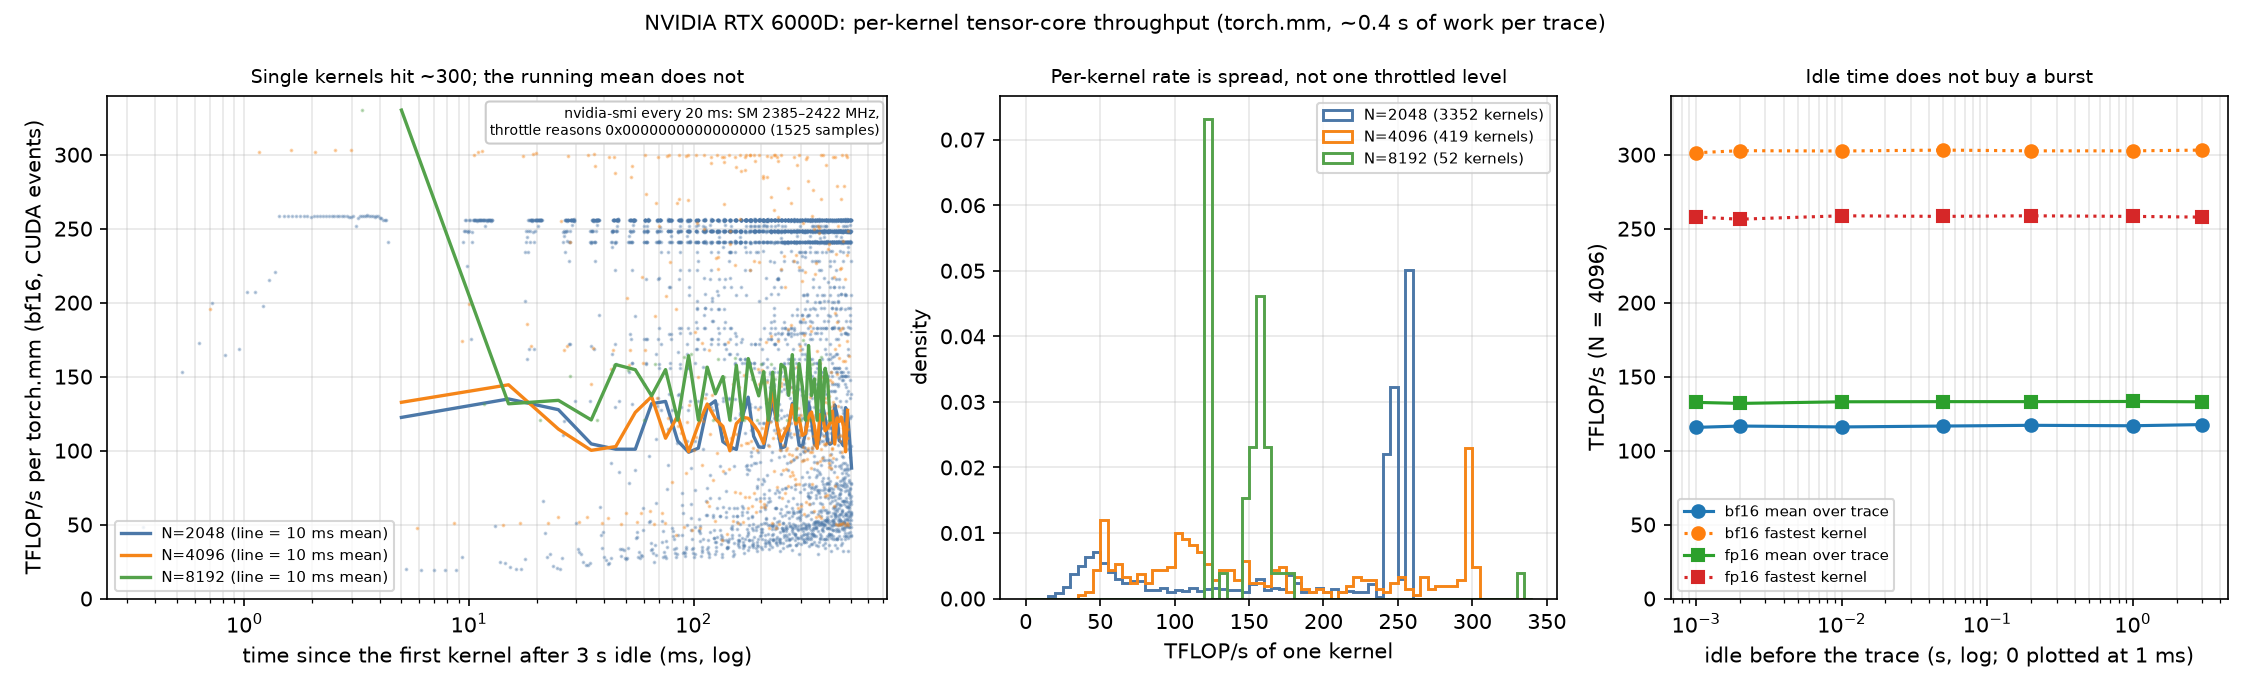
\includegraphics[width=\linewidth]{rtx6000d/burst.png}
\caption{逐 kernel 速度分布（双峰）与空闲时长扫描（无影响）。}
\label{fig:burst}
\end{figure}

\begin{findingbox}[：短 benchmark 测到的“峰值”是采样假象]
\texttt{peaks.json} 的 228.7~TFLOP/s，来自 30 次 75~µs 的 2048$^3$ 恰好落在一个快段里（共 2.3~ms）。能用来算 roofline 的是约 143~TFLOP/s 的持续值，
相对 5090 的 236 是 0.61 倍，cuBLAS 的 0.64 倍才是真实的算力比。在这张卡上，同一个 \texttt{a @ b} 计时 2~ms 和计时 8~s 会差 1.6 倍，
所以短 benchmark 要么跑够几百毫秒，要么报告中位数和分布。
\end{findingbox}

\begin{caveatbox}
限速发生在时钟以下、NVML 看不到的层面；没有 ncu 权限，具体机制（固件限流、tensor 管线发射限制）无法确认。
FlashAttention 0.43 倍再低一截，推测是它的 kernel 更短、更受快慢段影响，没有单独验证。
\end{caveatbox}

%==========================================================================================
\section{与理论模型的对照}
\label{sec:theory}

实验部分已经多次借用模型来解释数字。这一节把这些模型集中推一遍，看它们各自能预测什么，又在哪里失效。

\paragraph{分块流量与强度。} 对 $t_m\times t_n$ 的输出 tile，A 的每个元素被读 $\lceil N/t_n\rceil$ 次，B 被读 $\lceil M/t_m\rceil$ 次（\cref{eq:traffic}）。忽略 C 项，
\[
I \approx \frac{2MNK}{b\,(MKN/t_n + KNM/t_m)} = \frac{2}{b\,(1/t_m+1/t_n)} \overset{t_m=t_n=t}{=} \frac{t}{b}.
\]
因此 fp32 下 8、16、32、64、128 的 tile，强度约为 2、4、8、16、32~FLOP/B，与 \texttt{gemm\_ladder.jsonl} 中的 2.00、3.99、7.97、15.88、31.51 一致，差值来自 C 的 $4MN$ 项。
要达到 fp32 ridge 76.8~FLOP/B，按纯 DRAM 模型需要 $t\ge 4\times76.8\approx307$，也就是方形 tile 至少 320 左右。这在一个 block 的寄存器里放不下（见下段），
所以 GPU 上的 fp32 GEMM 要做到计算受限，\emph{必须依赖 L2}。bf16 下需要 $t\ge 2\times149.8\approx300$，道理相同。

\paragraph{片上容量决定 tile 上限。} Trainium 模型中，$4t_mt_n\le$ PSUM（2~MiB），所以 $t_mt_n\le 2^{19}$，即 512$\times$1024。
GPU 上累加器放在寄存器里，每 SM 的寄存器文件是 256~KB。一个 128$\times$128 fp32 block tile 的累加器是 64~KiB，2 个 block 同时驻留就占去寄存器文件的一半，
其余寄存器留给 A/B 片段和地址。这就是 vec4 每线程用 119--128 个寄存器、每 SM 恰好放 2 个 block 的由来。256$\times$256 的累加器是 256~KiB，已经等于整个寄存器文件，
必然 spill（实测 1108 字节 spill、3.09~TFLOP/s）。

\paragraph{一个寄存器的 occupancy 断崖。} 每 SM 有 65536 个寄存器，对 256 线程的 block，每 SM 能放 $\lfloor 65536/(256r)\rfloor$ 个 block。$r=128$ 时是 2 个，$r=129$ 时只剩 1 个。
本文的 vec4\_db 恰好踩在这条线上（129 个寄存器时 46.68，128 个时 49.44~TFLOP/s）。寄存器分配按 warp、以 8 为粒度取整，所以真实的断点可能略有不同，应以 occupancy API 的结果为准。

\paragraph{用流量模型预测性能。} 8192$^3$ 的 smem8：模型字节 550.02~GB，实测 3168.5~GFLOP/s，于是时间为 $2\cdot8192^3/3.1685\times10^{12}=0.347$~s，
隐含带宽 $550.02/0.347=1585$~GB/s，而 triad 实测是 1549~GB/s。同一个 kernel 在 4096$^3$ 的隐含带宽为 $68.79/(1.374\times10^{11}/7.172\times10^{12})=3.59$~TB/s，
介于 DRAM 与 L2 两个屋顶之间，说明工作集有一部分驻留在 L2。

\paragraph{Skinny GEMM。} $M\ll N,K$ 时 $I=\frac{2MNK}{b(MK+KN+MN)}\approx 2M/b$。fp32、M=1 时为 0.5~FLOP/B，屋顶是 $0.5\times1.549=0.77$~TFLOP/s；
实测最好的是我的 split-K（cold），0.546~TFLOP/s，即屋顶的 71\%。bf16 的屋顶翻倍。这也是 LLM decode 中权重量化（int8/int4）有效的原因：它直接减小了 $b$。

\paragraph{融合字节。} 非融合是 $4.25Y$，融合是 $0.25Y$，节省 $4Y$；只融合 ReLU+pool 则节省 $2Y$。batch 64、3$\times$3@112 C64 时，$4Y=784$~MiB，按 1.549~TB/s 算是 531~µs，实测省了 462~µs。
$2Y=392$~MiB 按 DRAM 算是 265~µs，实测却省了 351~µs，比按峰值换算的还多，因为 PyTorch 的 \texttt{F.relu} 和 \texttt{max\_pool2d} 本身没有跑到 DRAM 峰值。

\paragraph{脉动阵列。} 单个权重块的利用率在流水衔接时是 $\frac{M}{M+2P-2}$，串行加载权重时还要再加 $P$ 个周期，变成 $\frac{M}{M+3P-2}$。P=128、M=128 时为 $128/(128+382)=0.251$，与仿真一致。
放到 GPU tensor core 上，WMMA 在 1024$^3$ 只有 56.73~TFLOP/s，原因同样是工作量不足，填不满 170 个 SM 和每个 SM 里的 MMA 流水。

%==========================================================================================
\section{面试专题}

下面的问答按「先给结论，再给一个数字或推导，最后点出常见错答」来写，可以直接说出口。

\begin{iqbox}{为什么分块能提高 GEMM 性能？量化地说。}
因为分块让一个从 DRAM 取来的元素在片上被用很多次：$t\times t$ 的输出 tile，强度约为 $t/b$ FLOP/B。fp32 的 128 tile 是 31.5~FLOP/B，
而 RTX 5090 的 fp32 ridge 是 76.8，所以光靠 tile 还不够，还要靠 L2 的跨 block 复用。8192$^3$ 时 L2 帮不上忙，smem8 的性能可以用 $2.0~\text{FLOP/B}\times1.55~\text{TB/s}$ 精确预测，误差 2.3\%。

常见的错答是「分块是为了让数据放进 cache」。这句话没有说出复用次数与强度的关系，也解释不了 tile 大小的上限从哪里来。
\end{iqbox}

\begin{iqbox}{tile 越大越好吗？}
不是，强度随 tile 增大，但 tile 受片上容量约束：Trainium 上是 PSUM（模型中 2~MiB 把 tile 封顶在 512$\times$1024），GPU 上是寄存器文件和 shared memory。
我的热力图里，256$\times$256 的强度最高（62.1~FLOP/B），却只有 3.09~TFLOP/s，因为每 block 1024 线程，寄存器被压到 64 个，大量 spill；最快的是 64$\times$64（33.36）。

常见的错答是「越大越好，直到放不进 shared memory」。这忽略了寄存器、线程数和 occupancy 的约束，也忽略了小矩阵时 block 数不够（256$^3$ 只有 4 个 block）。
\end{iqbox}

\begin{iqbox}{occupancy 越高越好吗？}
不是。smem8/16 的理论 occupancy 是 100\%，只有 7--10~TFLOP/s；vec4 和 WMMA 只有 33\%，却最快。延迟既可以靠更多 warp（TLP）来藏，也可以靠每个线程里的独立指令（ILP）来藏。
FMA 微基准也说明了这一点：单链只有 89.0，16 条独立链达到 118.97~TFLOP/s。不过 occupancy 有断崖：vec4\_db 多用 1 个寄存器（129 个），每 SM 就从 2 个 block 掉到 1 个，慢了 6.6\%。

常见的错答是「occupancy 低说明 kernel 写得差，要尽量提高」。
\end{iqbox}

\begin{iqbox}{bank conflict 修掉之后为什么几乎没变快？}
因为瓶颈不在冲突，而在 shared 加载的\emph{指令数}。reg2d 有 4-way（B 读）和 8-way（A 转置写）冲突，修掉后只快 2.5\%（21.53$\to$22.07）；
它每 64 条 FMA 要配 16 条 LDS.32，换成 LDS.128 后只要 4 条，性能就到了 2.24 倍。所以应该先数指令，再修冲突。

常见的错答是「2D 分块慢，一定是 bank conflict」。这既没有量化，也没有验证。
\end{iqbox}

\begin{iqbox}{我测到 3.1~TB/s，超过了显存带宽，怎么回事？}
测到的其实是 L2 带宽。skinny GEMM 的 B 只有 64~MiB，反复调用时一直留在 96~MB 的 L2 里。每次调用前写一个 256~MiB 的缓冲区把 L2 冲掉，结果就降到 1093~GB/s（DRAM 峰值的 71\%）。
微基准也能印证：每数组 32~MiB 时 triad 为 5107~GB/s，从 64~MiB 起就掉到 1.65~TB/s 以下。

常见的错答是「GDDR7 的实际带宽比规格高」或者「计时有误」。这两种说法都没有想到 L2 容量和工作集的关系。
\end{iqbox}

\begin{iqbox}{conv+ReLU+maxpool 融合能省多少？}
省 $4Y$ 字节（$Y$ 是卷积输出），收益约为 $4Y$ 除以中间张量原本所在那一级存储的带宽。batch 64、3$\times$3@112 C64 时，模型流量从 1029.1 降到 245.1~MiB，时间从 4.230 降到 3.768~ms；
batch 8 时中间张量在 L2 里，只省 17--26~µs；卷积计算受限的层几乎省不了。

常见的错答是「融合减少了 kernel 启动次数，所以快」。启动开销只有几微秒，batch 64 省下的 462~µs 主要是 DRAM 流量。
\end{iqbox}

\begin{iqbox}{im2col、implicit GEMM、Winograd 怎么选？}
没有通用答案，要看形状和 GEMM 内核的质量。im2col 把卷积变成一个大 GEMM，可以直接复用 cuBLAS，代价是 $K_HK_W/s^2$ 倍的内存膨胀（conv1 为 12.25 倍、56.3~MiB），拷贝占 53--55\% 的时间。
implicit GEMM 在装 tile 时现场 gather，不膨胀，但前提是 GEMM 内核本身足够好，我的简单版本就比 im2col+cuBLAS 慢 1.7--11.8 倍。cuDNN 会按形状选算法；1$\times$1 卷积本来就是 GEMM，不需要 im2col。

常见的错答是「im2col 已经过时」或者「implicit GEMM 一定更快」。
\end{iqbox}

\begin{iqbox}{为什么 cuBLAS bf16 的误差比你的 WMMA 大 500 倍？}
因为输出格式不同，与累加精度无关：两者都用 fp32 累加。\texttt{torch.matmul} 对 bf16 输入输出 bf16，误差由输出舍入 $2^{-9}$ 主导（2.87e-3）；我的 kernel 输出 fp32（5.75e-6）。
比较精度时，必须固定输出格式和参考（这里是 fp64 在同一组舍入后的输入上计算）。

常见的错答是「cuBLAS 为了速度牺牲了精度」。
\end{iqbox}

\begin{iqbox}{Trainium 与 GPU 的编程模型差异，对 tiling 意味着什么？}
意味着同一个流量公式，在 Trainium 上是实际流量，在 GPU 上只是上界。Trainium 的 SBUF/PSUM 是显式管理的 scratchpad，DMA 由程序发起，HBM 和 SBUF 之间没有硬件 cache；
GPU 则有 L1/L2 硬件 cache，shared memory 只是可选的 scratchpad。本文 4096$^3$ 的 smem8 隐含带宽为 3.59~TB/s，远高于 DRAM，说明 L2 吸收了大部分重复读取。

常见的错答是「两者都是把 tile 搬到片上内存，没区别」。
\end{iqbox}

\subsection*{20 秒电梯陈述}
我把 CS149 A4 的 Trainium 分块问题搬到 RTX 5090 上，分两层来做：CPU 上是 SBUF/PSUM 流量模型和脉动阵列仿真，GPU 上是从 naive 到 tensor core 的 GEMM 阶梯和 conv 融合。
SGEMM 从 0.94 提升到 49.4~TFLOP/s，是 cuBLAS 的 78\%；WMMA 达到 cuBLAS fp16 的 86\%。最有说服力的一点是，工作集超过 L2 时，CPU 侧的流量公式预测 GPU 性能的误差只有 2.3\%。
融合则在中间张量溢出 L2 时省 11\%，在 L2 内几乎不省。

\subsection*{STAR 故事：一个寄存器的代价}
\begin{description}[leftmargin=1.5em]
  \item[Situation] 我在 float4 寄存器分块的 SGEMM（49.40~TFLOP/s）上加双缓冲，预期它能隐藏 shared-memory 的装载延迟。
  \item[Task] 要么证明双缓冲有效，要么解释它为什么没用。
  \item[Action] 第一次测下来，双缓冲版本反而慢了 6.6\%（46.68~TFLOP/s）。ncu 在容器里没有权限，我就改用 occupancy API 查资源，发现它用了 129 个寄存器，$256\times129>32768$，每 SM 只能放 1 个 block（8 个 warp）。
        对照 ptxas 输出后，我加了一个 \texttt{\_\_launch\_bounds\_\_(256,2)} 的版本，并在修改模板后重新编译。
  \item[Result] 寄存器降到 128（\texttt{launch\_bounds} 版本是 127），每 SM 回到 2 个 block，双缓冲版本回到 49.44~TFLOP/s，与单缓冲持平。
        结论是：BK=8 时每个 k 步只有 64 条 FMA，双缓冲能省的同步很少，它的寄存器和 smem 代价却可能直接让 occupancy 减半。从那以后，每改一个 kernel，我都先看 ptxas 的寄存器数和 occupancy。
\end{description}

%==========================================================================================
\section{局限}
下面这些限制说明了哪些结论不能外推，读数字时请一并考虑。
\begin{caveatbox}
\begin{itemize}
  \item 不能推出 Trainium 上的真实数字。加速器参数是假设的，GPU 上的数字只说明 GPU；两者共享的只是流量公式和容量约束的推理方式。
  \item 没有计数器级的证据。\texttt{ncu} 返回 \texttt{ERR\_NVGPUCTRPERM}，achieved occupancy、实测 DRAM 字节和 bank conflict 计数都没有测到。
        文中的 occupancy 是理论值，bank conflict 来自解析模型，DRAM 字节来自 tile 模型（不含 L2 复用的上界）。「L2 吸收了复用」是根据实测性能高于模型屋顶推断出来的，不是直接测量的结果。
  \item GPU 是共享机器。GPU 计时虽然在独占锁下进行，CPU 和 PCIe 仍与其他任务共享；GPU 时钟没有锁定（约 2.73~GHz 的有效时钟是反推出来的），不同轮次之间有约 1--3\% 的波动
        （例如 4096$^3$ 的 vec4 两次分别为 49.98 与 49.40~TFLOP/s）。
  \item 我的 conv kernel 是教学版本。direct 和 implicit GEMM 远慢于 cuDNN，不能据此推出「implicit GEMM 不如 im2col」。融合实验有意让融合与非融合共用同一个卷积计算，只比较中间张量的代价。
  \item double buffering 的结论只针对 BK=8、128$\times$128 的配置。更大的 BK、更深的流水（如多级 \texttt{cp.async}）或 warp 级分块，可能得出不同的结论。
  \item FP8 只测了 \texttt{torch.\_scaled\_mm} 的 e4m3、per-tensor scale、bf16 输出，没有测精度对模型质量的影响。
  \item CPU 部分的 Python 级分块测到的是解释器开销，不是 cache 效应；CPU 计时是在 4 核的共享机器上完成的。
\end{itemize}
\end{caveatbox}

%==========================================================================================
\section{结论}
这份报告想让读者带走的是下面几点：
\begin{enumerate}
  \item 分块的作用可以用一个公式说清：强度约为 $t/b$，而 tile 的上限由累加缓冲决定（Trainium 是 PSUM，GPU 是寄存器文件）。CPU 模型中 PSUM 把强度封顶在 315.08~FLOP/B；
        GPU 上 256$\times$256 的 tile 因为寄存器 spill，只有 3.09~TFLOP/s。
  \item 同一个流量公式在 GPU 上定量成立：8192$^3$ 的 smem8 隐含 DRAM 带宽为 1585~GB/s，与 triad 的 1549~GB/s 相差 2.3\%。工作集在 L2 内时，模型只是上界。
  \item SGEMM 阶梯中贡献最大的三步是合并访存（6.8 倍）、寄存器分块（2.6 倍）和 LDS.128（2.24 倍）；修 bank conflict 只贡献 2.5\%；双缓冲在本配置下持平，还可能因为多 1 个寄存器损失 6.6\%。
  \item 我的 kernel 达到 cuBLAS fp32 的 78.3\% 和 cuBLAS fp16 的 85.7\%。
  \item decode 形 GEMM 要看带宽：M=1 时最好的 fp32 实现只有 0.546~TFLOP/s（屋顶的 71\%），而且测量时必须冲掉 L2。
  \item 融合省的是中间张量的往返：中间张量在 L2 外时省 0.46~ms（11\%），在 L2 内只省 17~µs。Trainium 没有 L2 兜底，所以官方作业中的融合收益更接近前者。
\end{enumerate}

%==========================================================================================
\begin{thebibliography}{99}
\bibitem{williams2009} S. Williams, A. Waterman, D. Patterson. Roofline: An Insightful Visual Performance Model for Multicore Architectures. \emph{Communications of the ACM}, 52(4), 2009.
\bibitem{kung1982} H. T. Kung. Why Systolic Architectures? \emph{IEEE Computer}, 15(1), 1982.
\bibitem{jouppi2017} N. P. Jouppi et al. In-Datacenter Performance Analysis of a Tensor Processing Unit. \emph{ISCA}, 2017.
\bibitem{chen2017eyeriss} Y.-H. Chen, T. Krishna, J. Emer, V. Sze. Eyeriss: An Energy-Efficient Reconfigurable Accelerator for Deep Convolutional Neural Networks. \emph{IEEE JSSC}, 52(1), 2017.
\bibitem{goto2008} K. Goto, R. van de Geijn. Anatomy of High-Performance Matrix Multiplication. \emph{ACM TOMS}, 34(3), 2008.
\bibitem{volkov2008} V. Volkov, J. Demmel. Benchmarking GPUs to Tune Dense Linear Algebra. \emph{SC}, 2008.
\bibitem{volkov2010} V. Volkov. Better Performance at Lower Occupancy. \emph{GPU Technology Conference}, 2010.
\bibitem{jia2018} Z. Jia, M. Maggioni, B. Staiger, D. P. Scarpazza. Dissecting the NVIDIA Volta GPU Architecture via Microbenchmarking. arXiv:1804.06826, 2018.
\bibitem{chellapilla2006} K. Chellapilla, S. Puri, P. Simard. High Performance Convolutional Neural Networks for Document Processing. \emph{IWFHR}, 2006.
\bibitem{chetlur2014} S. Chetlur et al. cuDNN: Efficient Primitives for Deep Learning. arXiv:1410.0759, 2014.
\bibitem{lavin2016} A. Lavin, S. Gray. Fast Algorithms for Convolutional Neural Networks. \emph{CVPR}, 2016.
\bibitem{micikevicius2018} P. Micikevicius et al. Mixed Precision Training. \emph{ICLR}, 2018.
\bibitem{micikevicius2022} P. Micikevicius et al. FP8 Formats for Deep Learning. arXiv:2209.05433, 2022.
\bibitem{he2016} K. He, X. Zhang, S. Ren, J. Sun. Deep Residual Learning for Image Recognition. \emph{CVPR}, 2016.
\bibitem{simonyan2015} K. Simonyan, A. Zisserman. Very Deep Convolutional Networks for Large-Scale Image Recognition. \emph{ICLR}, 2015.
\bibitem{mccalpin1995} J. D. McCalpin. Memory Bandwidth and Machine Balance in Current High Performance Computers. \emph{IEEE TCCA Newsletter}, 1995.
\end{thebibliography}

\end{document}
